\chapter{\touist{} reference manual}\label{sec-language-reference}%mdk%mdk

\section{Language reference}

\subsection{Structure of a \touist file}\label{sec-structure-of-a-touist-file}%mdk%mdk
\begin{mdpre}%mdk
\noindent{\mdcolor{purple}\textless{}touist-file\textgreater{}}~::=~{\mdcolor{purple}\textless{}assign\textgreater{}}~{\mdcolor{purple}\textless{}touist-file\textgreater{}}\\
~~~~~~~~~~~~~~~~\textbar{}~{\mdcolor{purple}\textless{}formula\textgreater{}}~{\mdcolor{purple}\textless{}touist-file\textgreater{}}\\
~~~~~~~~~~~~~~~~\textbar{}~EOF%mdk
\end{mdpre}\noindent A \touist file is a whitespace-separated\footnote{\noindent A whitespace is a space, tab or newline.%mdk
\label{fn-whitespace}%mdk%mdk
} list of
assignments and formulas. Assignments are global and can be interleaved
with formulas as long as they are not nested in formulas (for local
variables, you can use \mdcode{{\mdcolor{navy}let}}; see Sec.~\ref{let-binding}). Comments begin
with "\mdcode{{\mdcolor{darkgreen};;}}". Two backslashes (\mdcode{\textbackslash{}\textbackslash{}}) in a formula will produce a new
line in the latex view.

\noindent\textbf{Note}.
The whitespace-separated list of formulas is actually going to be
converted to a conjunction; it avoids many intermediate \mdcode{and}.
\textbf{Warning:} each formula in this list is going to be put in
parentheses:%mdk
\begin{mdpre}%mdk
\noindent a~or~b\\
c~=\textgreater{}~a%mdk
\end{mdpre}\noindent will be translated to
\begin{mdpre}%mdk
\noindent(a~or~b)~and~(c~=\textgreater{}~a)%mdk
\end{mdpre}\label{newline-and-note}%mdk%mdk

\subsection{Variables}\label{sec-variables}%mdk%mdk

\noindent First, we describe what a variable is. Then, we detail how to assign
variables (with global or local assignments).%mdk

\subsubsection{Syntax of a variable}\label{sec-syntax-of-a-variable}%mdk%mdk
\begin{mdpre}%mdk
\noindent{\mdcolor{purple}\textless{}expr\textgreater{}}~::=~{\mdcolor{purple}\textless{}int\textgreater{}}\textbar{}{\mdcolor{purple}\textless{}float\textgreater{}}\textbar{}{\mdcolor{purple}\textless{}prop\textgreater{}}\textbar{}{\mdcolor{purple}\textless{}bool\textgreater{}}\textbar{}{\mdcolor{purple}\textless{}set\textgreater{}}\\
~~~~\textbar{}~"""{\mdcolor{purple}\textless{}formula-simple\textgreater{}}"""~{\mdcolor{darkgreen}\textless{}-~quoted~formula,~since~TouIST~\textgreater{}=~3.5.1}\\
{\mdcolor{purple}\textless{}var\textgreater{}}~::=~"\$"~TERM~~~~~~~~~~~~~~~~~~~~~~~~~~~~{\mdcolor{darkgreen}\textless{}-~simple-var}\\
~~~~\textbar{}~"\$"~TERM~"("~{\mdcolor{purple}\textless{}comma-list(\textless{}expr\textgreater{})\textgreater{}}~")"~~~{\mdcolor{darkgreen}\textless{}-~tuple-var}%mdk
\end{mdpre}
\begin{mddefinitions}%mdk

\mddefterm{\noindent{\bfseries Simple variable (\textquotedblleft{}simple-var\textquotedblright{})}}%mdk

\begin{mdbmarginx}{}{}{}{1.5em}%mdk
\begin{mddefdata}%mdk
A simple variable is of the form \mdcode{{\mdcolor{purple}\$my\_var}}. In a formula, a simple
variable is always expected to be a proposition or a
\mdref{quoted-formulas}{quoted formula}. In an expression, a simple
variable can contain an integer, a floating-point, a proposition, a boolean
or a set.
%mdk
\end{mddefdata}%mdk
\end{mdbmarginx}%mdk

\mddefterm{\noindent{\bfseries Tuple variable (can be seen as a \emph{predicate})}}%mdk

\begin{mdbmarginx}{}{}{}{1.5em}%mdk
\begin{mddefdata}%mdk
A tuple variable is a simple variable followed by a comma-separated list of
indexes in braces, e.g., \mdcode{{\mdcolor{purple}\$var}({\mdcolor{purple}\$i},a,{\mdcolor{purple}4})}. The leading variable (\mdcode{{\mdcolor{purple}\$var}})
must always contain a proposition. The nested indexes (e.g., \mdcode{{\mdcolor{purple}\$i}})
can be integers, floats, propositions or booleans.
%mdk
\end{mddefdata}%mdk
\end{mdbmarginx}%mdk

\begin{mdbmarginx}{}{}{}{1.5em}%mdk
\begin{mddefdata}%mdk
A tuple variable will always be expanded to a proposition or a
\mdref{quoted-formulas}{quoted formula}. For example, if
\mdcode{{\mdcolor{purple}\$var}=p} and \mdcode{{\mdcolor{purple}\$i}=q}, then it will expand to \mdcode{p(q,a,{\mdcolor{purple}4})}
%mdk
\end{mddefdata}%mdk
\end{mdbmarginx}%mdk

\begin{mdbmarginx}{}{}{}{1.5em}%mdk
\begin{mddefdata}%mdk
Tuple variables are not (yet) compatible with the set-builder construct (in
\ref{set-builder}). If one of the indexes is a set, the set will stay
as-is.%mdk
\end{mddefdata}%mdk
\end{mdbmarginx}%mdk
%mdk
\end{mddefinitions}%mdk

\noindent Here are some examples of variables:%mdk

\begin{mdcenter}%mdk
\begin{mdtabular}{2}{\dimeval{(\linewidth)/2}}{1ex}%mdk
\begin{tabular}{cc}\midrule
{\bfseries Simple-var}&{\bfseries Tuple-var}\\

\midrule
\mdcode{{\mdcolor{purple}\$N}}&\mdcode{{\mdcolor{purple}\$place}({\mdcolor{purple}\$number})}\\
\mdcode{{\mdcolor{purple}\$time}}&\mdcode{{\mdcolor{purple}\$action}({\mdcolor{purple}\$i},{\mdcolor{purple}\$j})}\\
\mdcode{{\mdcolor{purple}\$SIZE}}&\\
\mdcode{{\mdcolor{purple}\$is\_over}}&\\
\midrule
\end{tabular}\end{mdtabular}
%mdk
\end{mdcenter}%mdk

\subsubsection{Global assignment}\label{global-var}%mdk%mdk

\noindent We call \textquotedblleft{}global variables\textquotedblright{} any variable that is assigned at the same
depth as the subformulas of the \touist formula. A \touist formula is
the formula formed by the conjunction of each blank-separated \touist
statement (a blank is a newline, a space or a tabulation). For example,
in the following \touist formula:%mdk
\begin{mdpre}%mdk
\noindent a~and~(b~or~c)~d~e~=\textgreater{}~f~~~~\\
g~h~\textless{}=\textgreater{}~i\\
k~or~l\\
m%mdk
\end{mdpre}\noindent the subformulas \mdcode{a~and~(b~or~c)}, \mdcode{d}, \mdcode{e~or~f}, \mdcode{h~\textless{}=\textgreater{}~i},
\mdcode{k~or~l} are subformulas of the \touist formula but \mdcode{(b~or~c)} is not
(instead, it is a sub-subformula).

It is equivalent to%mdk
\noindent\noindent\[  (a \wedge (b \vee c)) \wedge (d) \wedge (e \rightarrow f) \wedge (g)
    \wedge (h \leftrightarrow i) \wedge (k \vee l) \wedge (m)
\]%mdk
\noindent This means that global variables cannot be nested in sub-subformulas;
they must appear at the same \textquotedblleft{}depth\textquotedblright{} as the subformulas. We cannot write
\mdcode{(a~or~({\mdcolor{purple}\$x}=b~{\mdcolor{purple}\$x}))} for example.

The assignment syntax is the following:%mdk
\begin{mdpre}%mdk
\noindent{\mdcolor{purple}\textless{}assign\textgreater{}}~::=~{\mdcolor{purple}\textless{}var\textgreater{}}~"="~({\mdcolor{purple}\textless{}expr\textgreater{}})~~~~~~{\mdcolor{darkgreen}\textless{}--~global~assignment}\\
{\mdcolor{purple}\textless{}expr\textgreater{}}~::=~{\mdcolor{purple}\textless{}int\textgreater{}}\textbar{}{\mdcolor{purple}\textless{}float\textgreater{}}\textbar{}{\mdcolor{purple}\textless{}prop\textgreater{}}\textbar{}{\mdcolor{purple}\textless{}bool\textgreater{}}\textbar{}{\mdcolor{purple}\textless{}set\textgreater{}}\\
~~~~\textbar{}~"""{\mdcolor{purple}\textless{}formula-simple\textgreater{}}"""~~~~~~~~~{\mdcolor{darkgreen}\textless{}--~TouIST~\textgreater{}=~3.5.1}%mdk
\end{mdpre}\noindent Global variables apply for the whole code, even if the assignment is
occurs after the use of the variable. This is because all global
assignments are evaluated before any formula.

The only case where the order of assignment is important is when you
want to use a variable in a global assignment expression. Global
assignments are sequentially evaluated, so the order of assignment
matters. For example:%mdk
\begin{mdpre}%mdk
\noindent{\mdcolor{purple}\$N}~=~{\mdcolor{purple}10}\\
{\mdcolor{purple}\$set}~=~{}[{\mdcolor{purple}1}..{\mdcolor{purple}\$N}]~~~~{\mdcolor{darkgreen};;~\$N~must~be~defined~before~\$set}%mdk
\end{mdpre}
\subsubsection{Local assignment (\mdcode{{\mdcolor{navy}let}} construct)}\label{let-binding}%mdk%mdk

\noindent Sometimes, you want to use the same result in multiple places and you
cannot use a global variable (presented in~\ref{global-var}) because of
nested formulas. The \mdcode{{\mdcolor{navy}let}} construct lets you create temporary
variables inside formulas:%mdk
\begin{mdpre}%mdk
\noindent{\mdcolor{purple}\textless{}let-assign\textless{}T\textgreater{}\textgreater{}}~::=\\
~~~~\textbar{}~"let"~{\mdcolor{purple}\textless{}var\textgreater{}}~"="~{\mdcolor{purple}\textless{}expr\textgreater{}}~":"~{\mdcolor{purple}\textless{}formula\textless{}T\textgreater{}\textgreater{}}~~~~~{\mdcolor{darkgreen}\textless{}--~local~assignment}\\
~~~~\textbar{}~"let"~{\mdcolor{purple}\textless{}comma-list(\textless{}var\textgreater{})\textgreater{}}~"="~{\mdcolor{purple}\textless{}comma-list(\textless{}expr\textgreater{})\textgreater{}}~":"~{\mdcolor{purple}\textless{}formula\textless{}T\textgreater{}\textgreater{}}\\
{\mdcolor{purple}\textless{}expr\textgreater{}}~::=~{\mdcolor{purple}\textless{}int\textgreater{}}\textbar{}{\mdcolor{purple}\textless{}float\textgreater{}}\textbar{}{\mdcolor{purple}\textless{}prop\textgreater{}}\textbar{}{\mdcolor{purple}\textless{}bool\textgreater{}}\textbar{}{\mdcolor{purple}\textless{}set\textgreater{}}%mdk
\end{mdpre}\noindent The \mdcode{{\mdcolor{navy}let}} assignment can only be used in formulas (detailed
in~\ref{sec-formulas}) and cannot be used in expressions (\mdcode{\textless{}expr\textgreater{}}, i.e.,
integer, floating-point, boolean or set expressions).

Example:%mdk
\begin{mdpre}%mdk
\noindent{\mdcolor{darkgreen};;~This~piece~of~code~has~no~actual~purpose}\\
{\mdcolor{purple}\$letters}~=~{}[a,b,c,d,e]\\
{\mdcolor{navy}bigand}~{\mdcolor{purple}\$letter},{\mdcolor{purple}\$number}~{\mdcolor{navy}in}~{\mdcolor{purple}\$letters},{}[{\mdcolor{purple}1}..{\mdcolor{navy}card}({\mdcolor{purple}\$letters})]:\\
~~has({\mdcolor{purple}\$letter},{\mdcolor{purple}\$number})~=\textgreater{}\\
~~{\mdcolor{navy}let}~{\mdcolor{purple}\$without\_letter}~=~{\mdcolor{navy}diff}({\mdcolor{purple}\$letters},{\mdcolor{purple}\$letter}):~{\mdcolor{darkgreen};;~keep~temorary~result}\\
~~{\mdcolor{navy}bigand}~{\mdcolor{purple}\$l1}~{\mdcolor{navy}in}~{\mdcolor{purple}\$without\_letter}:\\
~~~~~~p({\mdcolor{purple}\$letter})\\
~~{\mdcolor{navy}end}\\
{\mdcolor{navy}end}%mdk
\end{mdpre}\noindent You can also chain multiple variables in a single \mdcode{{\mdcolor{navy}let}}:
\begin{mdpre}%mdk
\noindent~~~~{\mdcolor{navy}let}~{\mdcolor{purple}\$E},{\mdcolor{purple}\$x},{\mdcolor{purple}\$y}~=~{}[{\mdcolor{purple}1}..{\mdcolor{purple}2}],{\mdcolor{purple}3},{\mdcolor{purple}4}:~...%mdk
\end{mdpre}
\noindent\textbf{Note}.
The scope of a variable assigned using \mdcode{{\mdcolor{navy}let}} is limited to the formula
that follows the colon (\mdcode{:}). If this formula is followed by a whitespace
and an other formula, the second formula will not be in the variable
scope. Example:%mdk
\begin{mdpre}%mdk
\noindent~~{\mdcolor{navy}let}~{\mdcolor{purple}\$v}={\mdcolor{purple}10}:~prop({\mdcolor{purple}\$v})\\
~~prop({\mdcolor{purple}\$v})~~~~{\mdcolor{darkgreen};;~error:~\$v~is~not~in~scope~anymore}%mdk
\end{mdpre}%mdk

\subsection{Propositions}\label{sec-propositions}%mdk%mdk
\begin{mdpre}%mdk
\noindent TERM~=~{}[\_0-9]*{}[a-zA-Z]{}[a-zA-Z\_0-9]*\\
{\mdcolor{purple}\textless{}expr\textgreater{}}~::=~{\mdcolor{purple}\textless{}int\textgreater{}}\textbar{}{\mdcolor{purple}\textless{}float\textgreater{}}\textbar{}{\mdcolor{purple}\textless{}prop\textgreater{}}\textbar{}{\mdcolor{purple}\textless{}bool\textgreater{}}\textbar{}{\mdcolor{purple}\textless{}set\textgreater{}}\\
{\mdcolor{purple}\textless{}prop\textgreater{}}~::=\\
~~~~\textbar{}~{\mdcolor{purple}\textless{}var\textgreater{}}\\
~~~~\textbar{}~TERM\\
~~~~\textbar{}~TERM~"("~{\mdcolor{purple}\textless{}comma-list(\textless{}expr\textgreater{})\textgreater{}}~")"%mdk
\end{mdpre}\noindent A simple proposition is a simple word that can contain numbers and the
underscore symbol ("\mdcode{\_}"). A tuple proposition (we can it as a
\emph{predicate}), of the form \mdcode{prop({\mdcolor{purple}1},{\mdcolor{purple}\$i},abc)}, must have indexes of type
integer, float, boolean or set.

\subsubsection{Tuple proposition containing a set}\label{tuple-prop-set}%mdk%mdk

\noindent A tuple proposition that is in an expression and that contains at least
one set in its indexes will be expanded to a set of the cartesian product
of the set indexes. This feature is called \textbf{set-building} and is
described in~\ref{set-builder} and only works in expressions (not in
formulas).%mdk

In the following table, the two right-columns show how the propositions
are expanded whether they are in an expression or in a formula:%mdk

\begin{mdcenter}%mdk
\begin{mdtabular}{3}{\dimeval{(\linewidth)/3}}{1ex}%mdk
\begin{tabular}{lll}\midrule
\multicolumn{1}{c}{{\bfseries Proposition}}&\multicolumn{1}{c}{{\bfseries is in a formula}}&\multicolumn{1}{c}{{\bfseries is in an expression}}\\

\midrule
\mdcode{p({}[a])}&\mdcode{p({}[a])}&\mdcode{p(a)}\\
\mdcode{p({}[a,b,c])}&\mdcode{p({}[a,b,c])}&\mdcode{{}[p(a),p(b),p(c)]}\\
\mdcode{p({}[a,b],{}[{\mdcolor{purple}1}..{\mdcolor{purple}2}])}&\mdcode{p({}[a,b],{}[{\mdcolor{purple}1}..{\mdcolor{purple}2}])}&\mdcode{{}[p(a,{\mdcolor{purple}1}),p(b,{\mdcolor{purple}1})}\\
&&~ \mdcode{p(a,{\mdcolor{purple}2}),p(b,{\mdcolor{purple}2})]}\\
\midrule
\end{tabular}\end{mdtabular}
%mdk
\end{mdcenter}%mdk

\subsection{Numeric expression}\label{sec-numeric-expression}%mdk%mdk

\noindent The available operations on integers and floats are \mdcode{+}, \mdcode{-}, \mdcode{*}, \mdcode{/},
\mdcode{{\mdcolor{purple}\$x}~{\mdcolor{navy}mod}~{\mdcolor{purple}\$y}} (modulo) and \mdcode{{\mdcolor{navy}abs}({\mdcolor{purple}\$x})} (absolute value). Parenthesis can
be used. The order of priority for the infix operators is:%mdk
\begin{mdtabular}{2}{\dimeval{(\linewidth)/2}}{1ex}%mdk
\begin{tabular}{lc}
\midrule
\emph{highest priority}&\mdcode{{\mdcolor{navy}mod}}\\
&\mdcode{*},\mdcode{/}\\
\emph{lowest priority}&\mdcode{+},\mdcode{-}\\
\midrule
\end{tabular}\end{mdtabular}

\noindent Here is the complete rule for numeric operators:%mdk
\begin{mdpre}%mdk
\noindent{\mdcolor{purple}\textless{}num-operation(\textless{}T\textgreater{})\textgreater{}}~::=\\
~~~~\textbar{}~{\mdcolor{purple}\textless{}T\textgreater{}}~"+"~{\mdcolor{purple}\textless{}T\textgreater{}}\\
~~~~\textbar{}~{\mdcolor{purple}\textless{}T\textgreater{}}~"-"~{\mdcolor{purple}\textless{}T\textgreater{}}\\
~~~~\textbar{}~~~~~"-"~{\mdcolor{purple}\textless{}T\textgreater{}}\\
~~~~\textbar{}~{\mdcolor{purple}\textless{}T\textgreater{}}~"*"~{\mdcolor{purple}\textless{}T\textgreater{}}\\
~~~~\textbar{}~{\mdcolor{purple}\textless{}T\textgreater{}}~"/"~{\mdcolor{purple}\textless{}T\textgreater{}}\\
{\mdcolor{purple}\textless{}num-operation-others(\textless{}T\textgreater{})\textgreater{}}~::=\\
~~~~\textbar{}~{\mdcolor{purple}\textless{}T\textgreater{}}~"mod"~{\mdcolor{purple}\textless{}T\textgreater{}}\\
~~~~\textbar{}~"abs("~{\mdcolor{purple}\textless{}T\textgreater{}}~")"%mdk
\end{mdpre}
\noindent\textbf{Note}.
Integer and float expressions cannot be mixed. It is necessary to cast
explicitely to the other type when the types are not matching. For
example, the expression \mdcode{{\mdcolor{purple}1}+{\mdcolor{purple}2.0}} is invalid and should be written
\mdcode{{\mdcolor{purple}1}+{\mdcolor{navy}int}({\mdcolor{purple}2.0})} (gives an integer) or \mdcode{{\mdcolor{navy}float}({\mdcolor{purple}1})+{\mdcolor{purple}2.0}} (gives a float).
Some operators are specific to integer or float types:%mdk

\begin{itemize}[noitemsep,topsep=\mdcompacttopsep]%mdk

\item\mdcode{{\mdcolor{navy}card}({}[a,b])} returns an integer,%mdk

\item\mdcode{{\mdcolor{navy}sqrt}({\mdcolor{purple}3})} returns a float.%mdk
%mdk
\end{itemize}%mdk%mdk

\subsubsection{Integers}\label{sec-integers}%mdk%mdk

\noindent An integer constant \mdcode{INT} is a number that satisfies the regular expression
\mdcode{{}[0-9]+}. Here is the rule for writting correct integer expressions:%mdk
\begin{mdpre}%mdk
\noindent{\mdcolor{purple}\textless{}int\textgreater{}}~::=\\
~~~~\textbar{}~"("~{\mdcolor{purple}\textless{}int\textgreater{}}~")"\\
~~~~\textbar{}~{\mdcolor{purple}\textless{}var\textgreater{}}\\
~~~~\textbar{}~INT\\
~~~~\textbar{}~num-operation({\mdcolor{purple}\textless{}int\textgreater{}})\\
~~~~\textbar{}~num-operation-others({\mdcolor{purple}\textless{}int\textgreater{}})\\
~~~~\textbar{}~"if"~{\mdcolor{purple}\textless{}bool\textgreater{}}~"then"~{\mdcolor{purple}\textless{}int\textgreater{}}~"else"~{\mdcolor{purple}\textless{}int\textgreater{}}~"end"\\
~~~~\textbar{}~"int("~({\mdcolor{purple}\textless{}int\textgreater{}}\textbar{}{\mdcolor{purple}\textless{}float\textgreater{}})~")"\\
~~~~\textbar{}~"card("~{\mdcolor{purple}\textless{}set\textgreater{}}~")"%mdk
\end{mdpre}
\subsubsection{Floats}\label{sec-floats}%mdk%mdk

\noindent A floating-point constant \mdcode{FLOAT} is a number that satisfies the regular
expression \mdcode{{}[0-9]+\textbackslash{}.{}[0-9]+}. The variants \mdcode{1.} or \mdcode{.1} are not accepted.
Here is the rule for writting correct integer expressions:%mdk
\begin{mdpre}%mdk
\noindent{\mdcolor{purple}\textless{}float\textgreater{}}~::=\\
~~~~\textbar{}~"("~{\mdcolor{purple}\textless{}float\textgreater{}}~")"\\
~~~~\textbar{}~{\mdcolor{purple}\textless{}var\textgreater{}}\\
~~~~\textbar{}~FLOAT\\
~~~~\textbar{}~num-operation({\mdcolor{purple}\textless{}float\textgreater{}})\\
~~~~\textbar{}~num-operation-others({\mdcolor{purple}\textless{}float\textgreater{}})\\
~~~~\textbar{}~"if"~{\mdcolor{purple}\textless{}bool\textgreater{}}~"then"~{\mdcolor{purple}\textless{}float\textgreater{}}~"else"~{\mdcolor{purple}\textless{}float\textgreater{}}~"end"\\
~~~~\textbar{}~"float("~({\mdcolor{purple}\textless{}int\textgreater{}}\textbar{}{\mdcolor{purple}\textless{}float\textgreater{}})~~")"\\
~~~~\textbar{}~"sqrt("~{\mdcolor{purple}\textless{}float\textgreater{}}~")"%mdk
\end{mdpre}
\subsection{Booleans}\label{sec-booleans}%mdk%mdk

\noindent The constants are \mdcode{{\mdcolor{navy}true}} and \mdcode{{\mdcolor{navy}false}}. The boolean connectors are $>$,
$<$, $\ge$ (\mdcode{\textgreater{}=}), $\le$ (\mdcode{\textless{}=}), $=$ (\mdcode{==}) and $\neq$ (\mdcode{!=}). The
operators that return a boolean are \mdcode{{\mdcolor{purple}\$P}~{\mdcolor{navy}subset}~{\mdcolor{purple}\$Q}}, \mdcode{{\mdcolor{navy}empty}({\mdcolor{purple}\$P})} and
\mdcode{p~{\mdcolor{navy}in}~{\mdcolor{purple}\$P}}:%mdk

\begin{mdcenter}%mdk
\begin{mdtabular}{3}{\dimeval{(\linewidth)/3}}{1ex}%mdk
\begin{tabular}{lcr}
\midrule
\mdcode{{\mdcolor{purple}\$P}~{\mdcolor{navy}subset}~{\mdcolor{purple}\$Q}}&$P \subseteq Q$&$P$ is a subset (or is included in) $Q$\\
\mdcode{{\mdcolor{navy}empty}({\mdcolor{purple}\$P})}&$P=\emptyset$&$P$ is an empty set\\
\mdcode{{\mdcolor{purple}\$i}~{\mdcolor{navy}in}~{\mdcolor{purple}\$P}}&$i \in P$&$i$ is an element of the set $P$\\
\midrule
\end{tabular}\end{mdtabular}
%mdk
\end{mdcenter}%mdk

\noindent Sets are detailed in~\ref{sec-sets}.%mdk

\noindent\textbf{Note}.
Booleans cannot be mixed with formulas. In a formula, the evaluation
(choosing true or false) is not done during the translation from \touist
to the \textquotedblleft{}solver-friendly\textquotedblright{} language. Conversely, a boolean expression must
be evaluable during the translation.%mdk
\label{dont-mix-bool-formula}%mdk%mdk

\noindent Parenthesis can be used in boolean expressions. The priority order for
booleans is:%mdk
\begin{mdtabular}{2}{\dimeval{(\linewidth)/2}}{1ex}%mdk
\begin{tabular}{lc}
\midrule
\emph{highest priority}&\mdcode{==},\mdcode{!=},\mdcode{\textless{}=},\mdcode{\textgreater{}=},\mdcode{\textless{}},\mdcode{\textgreater{}}, \mdcode{{\mdcolor{navy}in}}\\
&\mdcode{not}\\
&\mdcode{xor}\\
&\mdcode{and}\\
&\mdcode{or}\\
\emph{lowest priority}&\mdcode{=\textgreater{}}, \mdcode{\textless{}=\textgreater{}}\\
\midrule
\end{tabular}\end{mdtabular}

\noindent Note that \mdcode{=\textgreater{}} and \mdcode{\textless{}=\textgreater{}} associativity is evaluated from right to left.%mdk

Here is the full grammar rule for booleans:%mdk
\begin{mdpre}%mdk
\noindent{\mdcolor{purple}\textless{}bool\textgreater{}}~::=~"("~{\mdcolor{purple}\textless{}bool\textgreater{}}~")"\\
~~~~\textbar{}~{\mdcolor{purple}\textless{}var\textgreater{}}\\
~~~~\textbar{}~"true"\\
~~~~\textbar{}~"false"\\
~~~~\textbar{}~({\mdcolor{purple}\textless{}int\textgreater{}}\textbar{}{\mdcolor{purple}\textless{}float\textgreater{}}\textbar{}{\mdcolor{purple}\textless{}prop\textgreater{}}\textbar{}{\mdcolor{purple}\textless{}bool\textgreater{}})~"in"~{\mdcolor{purple}\textless{}set\textgreater{}}\\
~~~~\textbar{}~{\mdcolor{purple}\textless{}set\textgreater{}}~"subset"~{\mdcolor{purple}\textless{}set\textgreater{}}~~~~~~~~~~~~~~~~~~~~~{\mdcolor{darkgreen}\textless{}-~TouIST~\textgreater{}=~3.4.0}\\
~~~~\textbar{}~"subset("~{\mdcolor{purple}\textless{}set\textgreater{}}~","~{\mdcolor{purple}\textless{}set\textgreater{}}~")"\\
~~~~\textbar{}~"empty("~{\mdcolor{purple}\textless{}set\textgreater{}}~")"\\
~~~~\textbar{}~{\mdcolor{purple}\textless{}equality(\textless{}int\textgreater{}}\textbar{}{\mdcolor{purple}\textless{}float\textgreater{}}\textbar{}{\mdcolor{purple}\textless{}prop\textgreater{})\textgreater{}}\\
~~~~\textbar{}~{\mdcolor{purple}\textless{}order(\textless{}int\textgreater{}}\textbar{}{\mdcolor{purple}\textless{}float\textgreater{})\textgreater{}}\\
~~~~\textbar{}~{\mdcolor{purple}\textless{}connectors(\textless{}bool\textgreater{})\textgreater{}}\\
{\mdcolor{purple}\textless{}equality(\textless{}T\textgreater{})\textgreater{}}~::=\\
~~~~\textbar{}~{\mdcolor{purple}\textless{}T\textgreater{}}~"!="~{\mdcolor{purple}\textless{}T\textgreater{}}\\
~~~~\textbar{}~{\mdcolor{purple}\textless{}T\textgreater{}}~"=="~{\mdcolor{purple}\textless{}T\textgreater{}}\\
{\mdcolor{purple}\textless{}order(\textless{}T\textgreater{})\textgreater{}}~::=\\
~~~~\textbar{}~{\mdcolor{purple}\textless{}T\textgreater{}}~"\textgreater{}"~{\mdcolor{purple}\textless{}T\textgreater{}}\\
~~~~\textbar{}~{\mdcolor{purple}\textless{}T\textgreater{}}~"\textless{}"~{\mdcolor{purple}\textless{}T\textgreater{}}\\
~~~~\textbar{}~{\mdcolor{purple}\textless{}T\textgreater{}}~"\textless{}="~{\mdcolor{purple}\textless{}T\textgreater{}}\\
~~~~\textbar{}~{\mdcolor{purple}\textless{}T\textgreater{}}~"\textgreater{}="~{\mdcolor{purple}\textless{}T\textgreater{}}%mdk
\end{mdpre}
\subsection{Sets}\label{sec-sets}%mdk%mdk

\noindent Sets can contain anything (propositions, integers, floats,
booleans,~\mdref{quoted-formulas}{quoted formulas} or even other sets) as long
as all elements have the same type. There exists three ways of creating a
set:%mdk

\subsubsection{Sets defined by enumeration}\label{sec-sets-defined-by-enumeration}%mdk%mdk

\noindent$\{1,3,8,10\}$ can be written \mdcode{{}[{\mdcolor{purple}1},{\mdcolor{purple}2},{\mdcolor{purple}3}]}. Elements can be integers,
floats, propositions, booleans,~\mdref{quoted-formulas}{quoted formulas} or
sets (or a variable of these six types). The empty set $\emptyset$ is
denoted by \mdcode{{}[]}. Examples:%mdk
\begin{mdpre}%mdk
\noindent~~~~{}[{\mdcolor{purple}1},{\mdcolor{purple}2},{\mdcolor{purple}3}+{\mdcolor{purple}1}]\\
~~~~{}[a,b,p({\mdcolor{purple}1},v)]\\
~~~~{}[{}[{\mdcolor{purple}1},{\mdcolor{purple}2}],{}[{\mdcolor{purple}3},{\mdcolor{purple}4},{\mdcolor{purple}5}]]\\
~~~~{}["a~or~b",~"c~=\textgreater{}~d"]%mdk
\end{mdpre}
\subsubsection{Sets defined by a range}\label{sec-sets-defined-by-a-range}%mdk%mdk

\noindent$\{i~|~i=1,\dots,10\}$ can be written \mdcode{{}[{\mdcolor{purple}1}..{\mdcolor{purple}10}]}. Ranges can
be produced with both integer and float limits. For both integer and float
limits, the step is 1 (respectively 1.0). It is not possible to change the step for now.%mdk

\subsubsection{Set-builder notation (list comprehension)}\label{set-builder}%mdk%mdk

\noindent A set-builder expression is a set defined as
$\{p(x_1,...,x_n)~|~(x_1,...,x_n) \in S_1 \times ... \times S_n \}$,
which is the set of expressions based on the cartesian product of
the sets $S_1,...,S_n$. You can use the \textquotedblleft{}list comprehension\textquotedblright{} (since
version 3.5.2) to do that:%mdk
\begin{mdpre}%mdk
\noindent{}[p({\mdcolor{purple}\$i},{\mdcolor{purple}\$j},{\mdcolor{purple}\$k})~{\mdcolor{navy}for}~{\mdcolor{purple}\$i},{\mdcolor{purple}\$j},{\mdcolor{purple}\$k}~{\mdcolor{navy}in}~{\mdcolor{purple}\$S1},{\mdcolor{purple}\$S2},{\mdcolor{purple}\$S3}]%mdk
\end{mdpre}\noindent List comprehension allows you to generate sets containing any expression:
numbers, propositions and even formulas. In order to use formulas, you
must use the quoted notation (see Section~\ref{quoted-formulas}). The \mdcode{{\mdcolor{navy}when}}
keyword helps filter the generated elements (like in \mdcode{{\mdcolor{navy}bigand}} or
\mdcode{{\mdcolor{navy}bigor}}). Examples:
\begin{mdpre}%mdk
\noindent{}[{\mdcolor{purple}\$i}~{\mdcolor{navy}for}~{\mdcolor{purple}\$i}~{\mdcolor{navy}in}~{}[{\mdcolor{purple}1}..{\mdcolor{purple}100}]~{\mdcolor{navy}when}~{\mdcolor{purple}\$i}~{\mdcolor{navy}mod}~{\mdcolor{purple}3}~==~{\mdcolor{purple}0}]~{\mdcolor{darkgreen};;~set~of~integers}\\
{}[f({\mdcolor{purple}\$i},{\mdcolor{purple}\$j})~{\mdcolor{navy}for}~{\mdcolor{purple}\$i},{\mdcolor{purple}\$j}~{\mdcolor{navy}in}~{}[{\mdcolor{purple}1}..{\mdcolor{purple}3}],{}[a,b,c]]~~~~~{\mdcolor{darkgreen};;~set~of~propositions}\\
{}[f({\mdcolor{purple}1},{\mdcolor{purple}\$p})~{\mdcolor{navy}for}~{\mdcolor{purple}\$p}~{\mdcolor{navy}in}~{}[a,b,c,d]~{\mdcolor{navy}when}~{\mdcolor{purple}\$j}~!=~a]~{\mdcolor{darkgreen};;~set~of~propositions}\\
{}["{\mdcolor{purple}\$a}~and~{\mdcolor{purple}\$b}"~{\mdcolor{navy}for}~{\mdcolor{purple}\$a},{\mdcolor{purple}\$b}~{\mdcolor{navy}in}~{}[r,s],{}[x,y]]~~~~~{\mdcolor{darkgreen};;~set~of~quoted~formulas}%mdk
\end{mdpre}\noindent For simple list comprehension (without \mdcode{{\mdcolor{navy}when}}), you can use the
\textbf{condensed} syntax: \mdcode{f({\mdcolor{purple}1},{}[a,b],{}[{\mdcolor{purple}7}..{\mdcolor{purple}8}])} which is equivalent to
\mdcode{{}[f({\mdcolor{purple}1},{\mdcolor{purple}\$i},{\mdcolor{purple}\$j})~{\mdcolor{navy}for}~{\mdcolor{purple}\$i},{\mdcolor{purple}\$j}~{\mdcolor{navy}in}~{}[a,b],{}[{\mdcolor{purple}7}..{\mdcolor{purple}8}]]}.

\begin{mdcenter}%mdk
\begin{mdtabular}{2}{\dimeval{(\linewidth)/2}}{1ex}%mdk
\begin{tabular}{ll}
\midrule
\multicolumn{1}{|l}{List comprehension}&\multicolumn{1}{|l|}{\mdcode{{}[f({\mdcolor{purple}1},{\mdcolor{purple}\$i},{\mdcolor{purple}\$j})~{\mdcolor{navy}for}~{\mdcolor{purple}\$i},{\mdcolor{purple}\$j}~{\mdcolor{navy}in}~{}[a,b],{}[{\mdcolor{purple}7}..{\mdcolor{purple}8}]]}}\\
\multicolumn{1}{|l}{Condensed syntax}&\multicolumn{1}{|l|}{\mdcode{f({\mdcolor{purple}1},{}[a,b],{}[{\mdcolor{purple}7}..{\mdcolor{purple}8}])}}\\
\multicolumn{1}{|l}{Produced set}&\multicolumn{1}{|l|}{\mdcode{{}[f(1,a,7),f(1,a,8),f(1,b,7),f(1,b,8)]}`}\\
\midrule
\end{tabular}\end{mdtabular}
%mdk
\end{mdcenter}%mdk

\noindent\textbf{Important:} the set-builder feature only works in expressions and does
not work in formulas. In formulas, the proposition \mdcode{f({}[a,b])} will
simply produce \mdcode{f({}[a,b])}. This also means that you can debug your sets
by simply putting your set in a tuple proposition.%mdk

This notation is inspired from the concept of extension of a predicate (cf.
\href{https://en.wikipedia.org/wiki/Extension_(predicate_logic)}{wikipedia}).%mdk

\subsubsection{Operators using sets}\label{sec-operators-using-sets}%mdk%mdk

\noindent Some common set operators are available. Let $P$ and $Q$ denote two sets:%mdk

\begin{mdcenter}%mdk
\begin{mdtabular}{4}{\dimeval{(\linewidth)/4}}{1ex}%mdk
\begin{tabular}{llcl}\midrule
\multicolumn{1}{c}{{\bfseries Type}}&\multicolumn{1}{c}{{\bfseries Syntax}}&{\bfseries Math notation}&\multicolumn{1}{c}{{\bfseries Description}}\\

\midrule
\mdcode{{\mdcolor{purple}\textless{}set\textgreater{}}}&\mdcode{{\mdcolor{purple}\$P}~{\mdcolor{navy}inter}~{\mdcolor{purple}\$Q}}&$P \cap Q$&intersection\\
\mdcode{{\mdcolor{purple}\textless{}set\textgreater{}}}&\mdcode{{\mdcolor{purple}\$P}~{\mdcolor{navy}union}~{\mdcolor{purple}\$Q}}&$P \cup Q$&union\\
\mdcode{{\mdcolor{purple}\textless{}set\textgreater{}}}&\mdcode{{\mdcolor{purple}\$P}~{\mdcolor{navy}diff}~{\mdcolor{purple}\$Q}}&$P \setminus Q$&difference\\
\mdcode{{\mdcolor{purple}\textless{}set\textgreater{}}}&\mdcode{{\mdcolor{navy}powerset}({\mdcolor{purple}\$Q})}&$\mathcal{P}(Q)$&~\mdref{powerset}{powerset}\\
\mdcode{{\mdcolor{purple}\textless{}int\textgreater{}}}&\mdcode{{\mdcolor{navy}card}({\mdcolor{purple}\$S})}&$\vert S \vert$&cardinal\\
\mdcode{{\mdcolor{purple}\textless{}bool\textgreater{}}}&\mdcode{{\mdcolor{navy}empty}({\mdcolor{purple}\$P})}&$P=\emptyset$&set is empty\\
\mdcode{{\mdcolor{purple}\textless{}bool\textgreater{}}}&\mdcode{{\mdcolor{purple}\$e}~{\mdcolor{navy}in}~{\mdcolor{purple}\$P}}&$e \in P$&belongs to\\
\mdcode{{\mdcolor{purple}\textless{}bool\textgreater{}}}&\mdcode{{\mdcolor{purple}\$P}~{\mdcolor{navy}subset}~{\mdcolor{purple}\$Q}}&$P \subseteq Q$&is a subset or equal\\
\midrule
\end{tabular}\end{mdtabular}
%mdk
\end{mdcenter}%mdk

\noindent The three last operators of type \mdcode{\textless{}bool\textgreater{}} (\mdcode{{\mdcolor{navy}empty}}, \mdcode{{\mdcolor{navy}in}} and \mdcode{{\mdcolor{navy}subset}})
have also been described in the boolean section (\ref{sec-booleans}).%mdk

The priority on operators is:%mdk

\begin{mdcenter}%mdk
\begin{mdtabular}{2}{\dimeval{(\linewidth)/2}}{1ex}%mdk
\begin{tabular}{ll}
\midrule
highest priority&\mdcode{{\mdcolor{navy}inter}}\\
lowest priority&\mdcode{{\mdcolor{navy}union}}, \mdcode{{\mdcolor{navy}diff}}\\
\midrule
\end{tabular}\end{mdtabular}
%mdk
\end{mdcenter}%mdk

\noindent\textbf{Note}.
Up to \touist v3.2.3, the operators \mdcode{{\mdcolor{navy}inter}}, \mdcode{{\mdcolor{navy}union}}, \mdcode{{\mdcolor{navy}diff}} and
\mdcode{{\mdcolor{navy}subset}} were prefix operators (e.g., \mdcode{{\mdcolor{navy}inter}({\mdcolor{purple}\$A},{\mdcolor{purple}\$B})}). From v3.4.0
and later, these prefix operators are deprecated (but still usable).
Instead, we provide more human-friendly infix operators (e.g.,
\mdcode{{\mdcolor{purple}\$A}~{\mdcolor{navy}inter}~{\mdcolor{purple}\$B}}).%mdk%mdk

\paragraph{Powerset}\label{powerset}%mdk%mdk

\noindent The \mdcode{{\mdcolor{navy}powerset}({\mdcolor{purple}\$Q})} operator generates all possible subsets $S$ such
that $S \subseteq Q$. It is defined as%mdk
\noindent\noindent\[\mathcal{P}(Q) := \{S~|~S\subseteq Q\}
\]%mdk
\noindent The empty set is included in these subsets. Example:
\mdcode{{\mdcolor{navy}powerset}({}[{\mdcolor{purple}1},{\mdcolor{purple}2}])} generates \mdcode{{}[{}[],{}[{\mdcolor{purple}1}],{}[{\mdcolor{purple}2}],{}[{\mdcolor{purple}1},{\mdcolor{purple}2}]]}.

Here is the complete rule for sets:%mdk
\begin{mdpre}%mdk
\noindent{\mdcolor{purple}\textless{}set\textgreater{}}~::=~"("~{\mdcolor{purple}\textless{}set\textgreater{}}~")"\\
~~~~\textbar{}~{\mdcolor{purple}\textless{}var\textgreater{}}\\
~~~~\textbar{}~"{}["~{\mdcolor{purple}\textless{}comma-list(\textless{}int\textgreater{}}\textbar{}{\mdcolor{purple}\textless{}float\textgreater{}}\textbar{}{\mdcolor{purple}\textless{}prop\textgreater{}}\textbar{}{\mdcolor{purple}\textless{}bool\textgreater{})\textgreater{}}~"]"\\
~~~~\textbar{}~"{}[~{\mdcolor{purple}\textless{}int\textgreater{}}~".."~{\mdcolor{purple}\textless{}int\textgreater{}}~"]"~~~~~~{\mdcolor{darkgreen}\textless{}-~step~is~1}\\
~~~~\textbar{}~"{}[~{\mdcolor{purple}\textless{}float\textgreater{}}~".."~{\mdcolor{purple}\textless{}float\textgreater{}}~"]"~~{\mdcolor{darkgreen}\textless{}-~step~is~1.0}\\
~~~~\textbar{}~{\mdcolor{purple}\textless{}set\textgreater{}}~"inter"~{\mdcolor{purple}\textless{}set\textgreater{}}\\
~~~~\textbar{}~{\mdcolor{purple}\textless{}set\textgreater{}}~"union"~{\mdcolor{purple}\textless{}set\textgreater{}}\\
~~~~\textbar{}~{\mdcolor{purple}\textless{}set\textgreater{}}~"diff"~{\mdcolor{purple}\textless{}set\textgreater{}}\\
~~~~\textbar{}~"powerset("~{\mdcolor{purple}\textless{}set\textgreater{}}~")"%mdk
\end{mdpre}
\subsection{Formulas}\label{sec-formulas}%mdk%mdk

\subsubsection{Connectors}\label{sec-connectors}%mdk%mdk

\noindent A formula is a sequence of propositions (that can be variables) and connectors
$\neg p$ (\mdcode{not}), $\wedge$ (\mdcode{and}), $\vee$ (\mdcode{or}), $\oplus$ (\mdcode{xor}),
$\rightarrow$ (\mdcode{=\textgreater{}}) or $\leftrightarrow$ (\mdcode{\textless{}=\textgreater{}}).%mdk
\begin{mdpre}%mdk
\noindent{\mdcolor{purple}\textless{}connectors(\textless{}formula\textless{}T\textgreater{}\textgreater{})\textgreater{}}~::=\\
~~~~\textbar{}~~~~~"not"~{\mdcolor{purple}\textless{}T\textgreater{}}\\
~~~~\textbar{}~{\mdcolor{purple}\textless{}T\textgreater{}}~"and"~{\mdcolor{purple}\textless{}T\textgreater{}}\\
~~~~\textbar{}~{\mdcolor{purple}\textless{}T\textgreater{}}~"or"~{\mdcolor{purple}\textless{}T\textgreater{}}\\
~~~~\textbar{}~{\mdcolor{purple}\textless{}T\textgreater{}}~"xor"~{\mdcolor{purple}\textless{}T\textgreater{}}\\
~~~~\textbar{}~{\mdcolor{purple}\textless{}T\textgreater{}}~"=\textgreater{}"~{\mdcolor{purple}\textless{}T\textgreater{}}\\
~~~~\textbar{}~{\mdcolor{purple}\textless{}T\textgreater{}}~"\textless{}=\textgreater{}"~{\mdcolor{purple}\textless{}T\textgreater{}}%mdk
\end{mdpre}\noindent Parenthesis can be used in formulas in order to express priority. The
default operator priority is:
\begin{mdtabular}{2}{\dimeval{(\linewidth)/2}}{1ex}%mdk
\begin{tabular}{lc}
\midrule
\emph{highest priority}&\mdcode{not}\\
&\mdcode{xor}\\
&\mdcode{and}\\
&\mdcode{or}\\
&\mdcode{=\textgreater{}}, \mdcode{\textless{}=\textgreater{}}\\
\emph{lowest priority}&newline-\mdcode{and} (\ref{newline})\\
\midrule
\end{tabular}\end{mdtabular}

\noindent\textbf{Note}.
You can chain multiple variables in \mdcode{{\mdcolor{navy}bigand}} or \mdcode{{\mdcolor{navy}bigor}} by giving a
list of variables and sets. This will translate into nested
\mdcode{{\mdcolor{navy}bigand}}/\mdcode{{\mdcolor{navy}bigor}}. You can even use the value of outer variables in
inner set declarations:%mdk
\begin{mdpre}%mdk
\noindent{\mdcolor{navy}bigand}~{\mdcolor{purple}\$i},{\mdcolor{purple}\$j}~{\mdcolor{navy}in}~{}[{\mdcolor{purple}1}..{\mdcolor{purple}3}],~{}[{\mdcolor{purple}1}..{\mdcolor{purple}\$i}]:\\
~~~~p({\mdcolor{purple}\$i},{\mdcolor{purple}\$j})\\
{\mdcolor{navy}end}%mdk
\end{mdpre}%mdk

\subsubsection{Newline-\mdcode{and}}\label{newline}%mdk%mdk

\noindent As mentioned in a~\mdref{newline-and-note}{note} (first section), in \textbf{top-level}, a
new line (or any kind of white spaces) separating two formulas will be
translated into a lesser-priority \mdcode{and}. It is expressed in the grammar as:%mdk
\begin{mdpre}%mdk
\noindent{\mdcolor{purple}\textless{}formula(\textless{}T\textgreater{})\textgreater{}}:\\
~~\textbar{}~...\\
~~\textbar{}~{\mdcolor{purple}\textless{}T\textgreater{}}~("\textbackslash{}n"\textbar{}"~")~{\mdcolor{purple}\textless{}T\textgreater{}}~~~{\mdcolor{darkgreen}\textless{}-~newline/whitespace~in~top-level~is~an~'and'}%mdk
\end{mdpre}\noindent This notation is related to the idea of a set of formulas (premises). For
example, a new line would allow to express the separation of these two
formulas:
\noindent\noindent\[  \{a, a \Rightarrow b, \neg c\}
\]%mdk
\noindent You can write this either with
\begin{mdpre}%mdk
\noindent~~~~a\\
~~~~a~=\textgreater{}~b\\
~~~~not~c%mdk
\end{mdpre}\noindent or
\begin{mdpre}%mdk
\noindent~~~~a~a~=\textgreater{}~b~not~c%mdk
\end{mdpre}\noindent that are equivalent to
\noindent\noindent\[  a \wedge (a \Rightarrow b) \wedge (\neg c)
\]%mdk
\noindent The important thing to notice is that this \emph{whitespace-\mdcode{and}} has a
\textbf{lower priority} than any other connector.

\subsubsection{Generalized connectors}\label{sec-generalized-connectors}%mdk%mdk

\noindent Generalized connectors \mdcode{{\mdcolor{navy}bigand}}, \mdcode{{\mdcolor{navy}bigor}}, \mdcode{{\mdcolor{navy}exact}}, \mdcode{{\mdcolor{navy}atmost}} and
\mdcode{{\mdcolor{navy}atleast}} are also available for generalizing the formulas using sets. Here
is the rule for these:%mdk
\begin{mdpre}%mdk
\noindent{\mdcolor{purple}\textless{}generalized-connectors(\textless{}T\textgreater{})\textgreater{}}~::=\\
~~~~\textbar{}~"bigand"~{\mdcolor{purple}\textless{}comma-list(\textless{}var\textgreater{})\textgreater{}}~"in"~{\mdcolor{purple}\textless{}comma-list(\textless{}set\textgreater{})\textgreater{}}\\
~~~~~~~~~~~~~~~~~~~~~~~~~~~~~{}["when"~{\mdcolor{purple}\textless{}bool\textgreater{}}]~":"~{\mdcolor{purple}\textless{}T\textgreater{}}~"end"\\
~~~~\textbar{}~"bigor"~{\mdcolor{purple}\textless{}comma-list(\textless{}var\textgreater{})\textgreater{}}~"in"~{\mdcolor{purple}\textless{}comma-list(\textless{}set\textgreater{})\textgreater{}}\\
~~~~~~~~~~~~~~~~~~~~~~~~~~~~~{}["when"~{\mdcolor{purple}\textless{}bool\textgreater{}}]~":"~{\mdcolor{purple}\textless{}T\textgreater{}}~"end"\\
~~~~\textbar{}~"exact("~{\mdcolor{purple}\textless{}int\textgreater{}}~","~{\mdcolor{purple}\textless{}set\textgreater{}}~")"\\
~~~~\textbar{}~"atmost("~{\mdcolor{purple}\textless{}int\textgreater{}}~","~{\mdcolor{purple}\textless{}set\textgreater{}}~")"\\
~~~~\textbar{}~"atleast("~{\mdcolor{purple}\textless{}int\textgreater{}}~","~{\mdcolor{purple}\textless{}set\textgreater{}}~")"%mdk
\end{mdpre}
\paragraph{Bigand and bigor}\label{sec-bigand-and-bigor}%mdk%mdk

\noindent When multiple variables and sets are given, the \mdcode{{\mdcolor{navy}bigand}} and \mdcode{{\mdcolor{navy}bigor}}
operators will produce the \mdcode{and}/\mdcode{or} sequence for each possible couple of
value of each set (the set of couples is the Cartesian product of the given
sets). For example,%mdk

\begin{mdcenter}%mdk
\begin{mdtabular}{2}{\dimeval{(\linewidth)/2}}{1ex}%mdk
\begin{tabular}{ll}\midrule
{\bfseries The formula}&\multicolumn{1}{|c}{{\bfseries expands to\dots{}}}\\

\midrule
$\bigwedge\limits_{\substack{i\in \{1,...,2\}\\j \in \{a,b\}}} p_{i,j}$&\multicolumn{1}{|l}{$p_{1,a} \wedge p_{1,b} \wedge p_{2,a} \wedge p_{2,b}$}\\
\midrule
\mdcode{{\mdcolor{navy}bigand}~{\mdcolor{purple}\$i},{\mdcolor{purple}\$j}~{\mdcolor{navy}in}~{}[{\mdcolor{purple}1}..{\mdcolor{purple}2}],{}[a,b]:}&\multicolumn{1}{|l}{\mdcode{p({\mdcolor{purple}1},a)~and~p({\mdcolor{purple}1},b)~}}\\
\mdcode{p({\mdcolor{purple}\$i},{\mdcolor{purple}\$j})}&\multicolumn{1}{|l}{\mdcode{and~p({\mdcolor{purple}2},a)~and~p({\mdcolor{purple}2},b)}}\\
\mdcode{{\mdcolor{navy}end}}&\multicolumn{1}{|l}{}\\
\midrule
\end{tabular}\end{mdtabular}

%mdk
\end{mdcenter}%mdk

\noindent The \mdcode{{\mdcolor{navy}when}} is optional and allows us to apply a condition to each
couple of valued variable.%mdk

On the following two examples, the math expression is given on the left
and the matching \touist code is given on the right:%mdk
\begin{mdtabular}{2}{\dimeval{(\linewidth-\dimwidth{0.30})/1}}{0pt}%mdk
\begin{tabular}{ll}

\begin{mdcolumn}%mdk
\begin{mdblock}{width=\dimwidth{0.30}}%mdk
\noindent$\bigwedge\limits_{\substack{i\in [1..n]\\j \in [a,b,c]}} p_{i,j}$%mdk%mdk
\end{mdblock}%mdk
\end{mdcolumn}%mdk
&
\begin{mdcolumn}%mdk
\begin{mdblock}{width=\dimavailable}%mdk
\begin{mdpre}%mdk
\noindent{\mdcolor{navy}bigand}~{\mdcolor{purple}\$i},{\mdcolor{purple}\$j}~{\mdcolor{navy}in}~{}[{\mdcolor{purple}1}..{\mdcolor{purple}\$n}],{}[a,b,c]:\\
~~~~p({\mdcolor{purple}\$i},{\mdcolor{purple}\$j})\\
{\mdcolor{navy}end}%mdk
\end{mdpre}%mdk
\end{mdblock}%mdk
\end{mdcolumn}%mdk
\\
\end{tabular}\end{mdtabular}
\begin{mdtabular}{2}{\dimeval{(\linewidth-\dimwidth{0.30})/1}}{0pt}%mdk
\begin{tabular}{ll}

\begin{mdcolumn}%mdk
\begin{mdblock}{width=\dimwidth{0.30}}%mdk
\noindent$\bigvee\limits_{\substack{v\in [A,B,C]\\x \in [1..9]\\y\in[3..4]\\x \ne y \\ x \ne A\\}} v_{x,y}$%mdk%mdk
\end{mdblock}%mdk
\end{mdcolumn}%mdk
&
\begin{mdcolumn}%mdk
\begin{mdblock}{width=\dimavailable}%mdk
\begin{mdpre}%mdk
\noindent{\mdcolor{navy}bigor}~{\mdcolor{purple}\$v},{\mdcolor{purple}\$x},{\mdcolor{purple}\$y}\\
~~~~~~{\mdcolor{navy}in}~{}[A,B,C],{}[{\mdcolor{purple}1}..{\mdcolor{purple}9}],{}[{\mdcolor{purple}3}..{\mdcolor{purple}4}]\\
~~~~~~{\mdcolor{navy}when}~{\mdcolor{purple}\$v}!=A~and~{\mdcolor{purple}\$x}!={\mdcolor{purple}\$y}:\\
~~~~{\mdcolor{purple}\$v}({\mdcolor{purple}\$x})\\
{\mdcolor{navy}end}%mdk
\end{mdpre}%mdk
\end{mdblock}%mdk
\end{mdcolumn}%mdk
\\
\end{tabular}\end{mdtabular}

\paragraph{Special cases for quantifier elimination}\label{sec-special-cases-for-quantifier-elimination}%mdk%mdk

\noindent Here is the list of \textquotedblleft{}limit\textquotedblright{} cases where \mdcode{{\mdcolor{navy}bigand}} and \mdcode{{\mdcolor{navy}bigor}} will produce
special results:%mdk

\begin{itemize}[noitemsep,topsep=\mdcompacttopsep]%mdk

\item In \mdcode{{\mdcolor{navy}bigand}}, if a set is empty then \mdcode{{\mdcolor{navy}Top}} is produced%mdk

\item In \mdcode{{\mdcolor{navy}bigand}}, if the \mdcode{{\mdcolor{navy}when}} condition is always false then \mdcode{{\mdcolor{navy}Top}}
is produced%mdk

\item In \mdcode{{\mdcolor{navy}bigor}}, if a set is empty then \mdcode{{\mdcolor{navy}Bot}} is produced%mdk

\item In \mdcode{{\mdcolor{navy}bigor}}, if the \mdcode{{\mdcolor{navy}when}} condition is always false then \mdcode{{\mdcolor{navy}Bot}} is
produced%mdk
%mdk
\end{itemize}%mdk

\noindent These behaviors come from the idea of quantification behind the
\mdcode{{\mdcolor{navy}bigand}} and \mdcode{{\mdcolor{navy}bigor}} operators:%mdk

\begin{mdcenter}%mdk
\begin{mdtabular}{3}{\dimeval{(\linewidth-\dimwidth{0.25})/2}}{1ex}%mdk
\begin{tabular}{lcl}
Universal quantification&\mdinline{width=\dimwidth{0.25}}{$\forall x \in S, p(x)$}&\mdcode{{\mdcolor{navy}bigand}~{\mdcolor{purple}\$x}~{\mdcolor{navy}in}~{\mdcolor{purple}\$S}:~p({\mdcolor{purple}\$x})~{\mdcolor{navy}end}}\\
\midrule
Existential quantification&\mdinline{width=\dimwidth{0.25}}{$\exists x \in S, p(x)$}&\mdcode{{\mdcolor{navy}bigor}~{\mdcolor{purple}\$x}~{\mdcolor{navy}in}~{\mdcolor{purple}\$S}:~p({\mdcolor{purple}\$x})~{\mdcolor{navy}end}}\\
\end{tabular}\end{mdtabular}
%mdk
\end{mdcenter}%mdk

\noindent The following properties on quantifiers hold:%mdk
\label{}%mdk
\noindent\mdmathtag{(1)}
\noindent\[\begin{aligned}
\forall x \in \emptyset, p(x) \quad \equiv \quad \top \\
\exists x \in \emptyset, p(x) \quad \equiv \quad \bot
\end{aligned}
\]%mdk
\noindent which helps understand why \mdcode{{\mdcolor{navy}Top}} and \mdcode{{\mdcolor{navy}Bot}} are produced.

\noindent\textbf{Todo}.
Clarify this explanation.%mdk%mdk

\paragraph{Exact, atmost and atleast}\label{sec-exact-atmost-and-atleast}%mdk%mdk

\noindent The \touist language provides some specialized operators, namely
\mdcode{{\mdcolor{navy}exact}}, \mdcode{{\mdcolor{navy}atmost}} and \mdcode{{\mdcolor{navy}atleast}}. In some cases, these operators can
drastically lower the size of some formulas. The syntax of these constructs
is:%mdk

\begin{mdcenter}%mdk
\begin{mdtabular}{2}{\dimeval{(\linewidth)/2}}{1ex}%mdk
\begin{tabular}{cl}\midrule
{\bfseries Math notation}&\multicolumn{1}{c}{{\bfseries\touist syntax}}\\

\midrule
$\leqslant_{x\in P}^k x$&\mdcode{{\mdcolor{navy}atmost}({\mdcolor{purple}\$k},{\mdcolor{purple}\$P})}\\
$\geqslant_{x\in P}^k x$&\mdcode{{\mdcolor{navy}atleast}({\mdcolor{purple}\$k},{\mdcolor{purple}\$P})}\\
${<>}_{x\in P}^k x$&\mdcode{{\mdcolor{navy}exact}({\mdcolor{purple}\$k},{\mdcolor{purple}\$P})}\\
\midrule
\end{tabular}\end{mdtabular}
%mdk
\end{mdcenter}%mdk

\noindent Let $P$ be a set of propositions, $x$ a proposition and $k$ a positive
integer. Then:%mdk

\begin{itemize}[noitemsep,topsep=\mdcompacttopsep]%mdk

\item$\leqslant_{x\in P}^k x$ represents "at any time, at most $k$
propositions $x \in P$ must be true"%mdk

\item$\geqslant_{x\in P}^k x$ represents "at any time, at least $k$
propositions $x \in P$ must be true"%mdk

\item${<>}_{x\in P}^k x$ represents "at any time, exactly $k$ propositions
$x \in P$ must be true"%mdk
%mdk
\end{itemize}%mdk

\noindent These operators are extremely expensive in the sense that they produce formulas
with an exponential size. For example, \mdcode{{\mdcolor{navy}exact}({\mdcolor{purple}5},p({}[{\mdcolor{purple}1}..{\mdcolor{purple}20}])}
will produce a disjunction of $\binom{20}{5} = 15 504$ conjunctions.%mdk

\noindent\textbf{Note}.
The notation \mdcode{p({}[{\mdcolor{purple}1}..{\mdcolor{purple}20}])} is called \textquotedblleft{}set-builder\textquotedblright{} and is defined
in~\ref{set-builder}. Using this syntax, the formula \mdcode{{\mdcolor{navy}exact}({\mdcolor{purple}5},p({}[{\mdcolor{purple}1}..{\mdcolor{purple}20}])}
is equivalent to%mdk
\noindent\noindent\[{<>}_{x\in P}^k p(x)
\]%mdk%mdk

\begin{mdbmarginx}{1ex}{0pt}{1ex}{0pt}%mdk
\noindent\textbf{Example~1.} \mdbr
\mdcode{{\mdcolor{navy}exact}({\mdcolor{purple}2},{}[a,b,c])} is equivalent to%mdk
\noindent\noindent\[\left(a \wedge b \wedge \neg c\right) \vee \left(a \wedge \neg b \wedge c\right) \vee \left(\neg a \wedge b \wedge c\right)
\]%mdk%mdk
\end{mdbmarginx}%mdk

\paragraph{Special cases for operator elimination}\label{sec-special-cases-for-operator-elimination}%mdk%mdk

\noindent The following table sums up the various \textquotedblleft{}limit\textquotedblright{} cases that may not be obvious.
In this table, $k$ is a positive integer and $P$ is a set of propositions.%mdk

\begin{mdcenter}%mdk
\begin{mdtabular}{4}{\dimeval{(\linewidth)/4}}{1ex}%mdk
\begin{tabular}{lccl}\midrule
\multicolumn{1}{c}{{\bfseries}}&\multicolumn{1}{|c}{{\bfseries\mdcode{{\mdcolor{purple}\$k}}}}&\multicolumn{1}{|c}{{\bfseries\mdcode{{\mdcolor{purple}\$P}}}}&\multicolumn{1}{|c}{{\bfseries Gives}}\\

\midrule
\mdcode{{\mdcolor{navy}exact}({\mdcolor{purple}\$k},{\mdcolor{purple}\$P})}&\multicolumn{1}{|c}{$k=0$}&\multicolumn{1}{|c}{$P=\emptyset$}&\multicolumn{1}{|l}{\mdcode{{\mdcolor{navy}Top}}}\\
&\multicolumn{1}{|c}{$k=0$}&\multicolumn{1}{|c}{$P\neq\emptyset$}&\multicolumn{1}{|l}{\mdcode{{\mdcolor{navy}bigand}~{\mdcolor{purple}\$p}~{\mdcolor{navy}in}~{\mdcolor{purple}\$P}:~not~{\mdcolor{purple}\$p}~{\mdcolor{navy}end}}}\\
&\multicolumn{1}{|c}{$k>0$}&\multicolumn{1}{|c}{$\vert P\vert=k$}&\multicolumn{1}{|l}{\mdcode{{\mdcolor{navy}bigand}~{\mdcolor{purple}\$p}~{\mdcolor{navy}in}~{\mdcolor{purple}\$P}:~{\mdcolor{purple}\$p}~{\mdcolor{navy}end}}}\\
\mdcode{{\mdcolor{navy}atleast}({\mdcolor{purple}\$k},{\mdcolor{purple}\$P})}&\multicolumn{1}{|c}{$k=0$}&\multicolumn{1}{|c}{any}&\multicolumn{1}{|l}{\mdcode{{\mdcolor{navy}Top}}}\\
&\multicolumn{1}{|c}{$k=1$}&\multicolumn{1}{|c}{any}&\multicolumn{1}{|l}{\mdcode{{\mdcolor{navy}bigor}~{\mdcolor{purple}\$p}~{\mdcolor{navy}in}~{\mdcolor{purple}\$P}:~{\mdcolor{purple}\$p}~{\mdcolor{navy}end}}}\\
&\multicolumn{1}{|c}{$k>0$}&\multicolumn{1}{|c}{$\emptyset$}&\multicolumn{1}{|l}{\mdcode{{\mdcolor{navy}Bot}} (subcase of next row)}\\
&\multicolumn{1}{|c}{$k>0$}&\multicolumn{1}{|c}{$\vert P\vert<k$}&\multicolumn{1}{|l}{\mdcode{{\mdcolor{navy}Bot}}}\\
&\multicolumn{1}{|c}{$k>0$}&\multicolumn{1}{|c}{$\vert P\vert=k$}&\multicolumn{1}{|l}{\mdcode{{\mdcolor{navy}bigand}~{\mdcolor{purple}\$p}~{\mdcolor{navy}in}~{\mdcolor{purple}\$P}:~{\mdcolor{purple}\$p}~{\mdcolor{navy}end}}}\\
\mdcode{{\mdcolor{navy}atmost}({\mdcolor{purple}\$k},{\mdcolor{purple}\$P})}&\multicolumn{1}{|c}{$k=0$}&\multicolumn{1}{|c}{$\emptyset$}&\multicolumn{1}{|l}{\mdcode{{\mdcolor{navy}Top}} (subcase of next row)}\\
&\multicolumn{1}{|c}{$k=0$}&\multicolumn{1}{|c}{any}&\multicolumn{1}{|l}{\mdcode{{\mdcolor{navy}Top}}}\\
\midrule
\end{tabular}\end{mdtabular}
%mdk
\end{mdcenter}%mdk

\noindent How to read the table: for example, the row where $k>0$ and
$\vert P\vert<k$ should be read "when using \mdcode{{\mdcolor{navy}atleast}}, all couples
$(k,P) \in \{(k,P)|k>0,\vert P\vert<k\}$ will produce the special case
\mdcode{{\mdcolor{navy}Top}}".%mdk

\subsubsection{Propositional logic formulas}\label{sec-propositional-logic-formulas}%mdk%mdk

\noindent The constants $\top$ (\mdcode{{\mdcolor{navy}Top}}) and $\bot$ (\mdcode{{\mdcolor{navy}Bot}}) allow us to express
the \textquotedblleft{}always true\textquotedblright{} and \textquotedblleft{}always false\textquotedblright{}. Here is the complete grammar:%mdk
\begin{mdpre}%mdk
\noindent{\mdcolor{purple}\textless{}formula-simple\textgreater{}}~::=\\
~~~~\textbar{}~"Top"\\
~~~~\textbar{}~"Bot"\\
~~~~\textbar{}~{\mdcolor{purple}\textless{}prop\textgreater{}}\\
~~~~\textbar{}~{\mdcolor{purple}\textless{}var\textgreater{}}\\
~~~~\textbar{}~{\mdcolor{purple}\textless{}formula(\textless{}formula-simple\textgreater{})\textgreater{}}\\
\\
{\mdcolor{purple}\textless{}formula(\textless{}T\textgreater{})\textgreater{}}~::=\\
~~~~\textbar{}~"("~{\mdcolor{purple}\textless{}T\textgreater{}}~")"\\
~~~~\textbar{}~"if"~{\mdcolor{purple}\textless{}bool\textgreater{}}~"then"~{\mdcolor{purple}\textless{}T\textgreater{}}~"else"~{\mdcolor{purple}\textless{}T\textgreater{}}~"end"\\
~~~~\textbar{}~{\mdcolor{purple}\textless{}connectors(\textless{}T\textgreater{})\textgreater{}}\\
~~~~\textbar{}~{\mdcolor{purple}\textless{}generalized-connectors(\textless{}T\textgreater{})\textgreater{}}\\
~~~~\textbar{}~{\mdcolor{purple}\textless{}let-assign(\textless{}T\textgreater{})\textgreater{}}\\
%mdk
\end{mdpre}
\subsubsection{SMT formulas}\label{sec-smt-formulas}%mdk%mdk

\noindent The \touist language also accepts formulas of the Satisfiability Modulo Theory (SMT).
To use the \mdcode{touist} program with SMT formulas, see Section~\ref{usage-smt}.%mdk

\noindent\textbf{Todo}.
Describe the SMT language%mdk%mdk

\subsubsection{QBF formulas}\label{sec-qbf-formulas}%mdk%mdk

\noindent The \touist language accepts Quantified Boolean Formulas (QBF). Using
the \mdcode{--qbf} and \mdcode{--solve} flags (in \mdcode{touist}) or the QBF selector (in the
graphical interface), you can solve QBF problems with existential and
universal quantifiers over boolean values. This logic is basically the
same as the SAT grammar, except for two new operators $\exists$
(\mdcode{{\mdcolor{navy}exists}}) and $\forall$ (\mdcode{{\mdcolor{navy}forall}}):%mdk
\begin{mdpre}%mdk
\noindent{\mdcolor{purple}\textless{}formula-qbf\textgreater{}}~::=\\
~~~~{}[...]\\
~~~~\textbar{}~"exists"~{\mdcolor{purple}\textless{}comma-list(\textless{}prop\textgreater{}}\textbar{}{\mdcolor{purple}\textless{}var\textgreater{})\textgreater{}}~{}[{\mdcolor{purple}\textless{}for\textgreater{}}]~":"~{\mdcolor{purple}\textless{}formula-qbf\textgreater{}}\\
~~~~\textbar{}~"forall"~{\mdcolor{purple}\textless{}comma-list(\textless{}prop\textgreater{}}\textbar{}{\mdcolor{purple}\textless{}var\textgreater{})\textgreater{}}~{}[{\mdcolor{purple}\textless{}for\textgreater{}}]~":"~{\mdcolor{purple}\textless{}formula-qbf\textgreater{}}\\
\\
{\mdcolor{purple}\textless{}for\textgreater{}}~::=~"for"~{\mdcolor{purple}\textless{}var\textgreater{}}~"in"~{\mdcolor{purple}\textless{}set\textgreater{}}%mdk
\end{mdpre}\noindent One quantifier can quantify over multiple propositions. For example:
\begin{mdpre}%mdk
\noindent~~~~{\mdcolor{navy}forall}~e,d:~({\mdcolor{navy}exists}~a,b:~a~=\textgreater{}~b)~=\textgreater{}~(e~and~{\mdcolor{navy}forall}~c:~e~=\textgreater{}~c)%mdk
\end{mdpre}\noindent\noindent\[\forall e. \forall d. (\exists a. \exists b. (a \Rightarrow b)) \Rightarrow (e \wedge \forall c. (e \Rightarrow c))
\]%mdk

\paragraph{Free variables}\label{sec-free-variables}%mdk%mdk

\noindent Any free variable (i.e., not quantified) will be existentially quantified
in an inner-most way. For example, $\forall a. a \wedge b$ will become
$\forall a. \forall b. (a \wedge b)$.%mdk

\paragraph{Renaming during the prenex transformation}\label{sec-renaming-during-the-prenex-transformation}%mdk%mdk

\noindent Using the rules for transforming an arbitrary formula into prenex form
requires sometimes some renaming. For example, $(\forall a. a) \wedge a$
must be transformed into $\forall a_1. (a_1 \wedge a))$.%mdk

Sometimes, the renaming is not possible. For example, in
$\forall a. (\exists a. a)$, we cannot guess which quantifier the
rightmost $a$ should be bound to. In this case, \mdcode{touist} will give and
error.%mdk

Also, the use of the whitespace-as-formula-separator can lead to some
misunderstanding. For example, in formula%mdk
\begin{mdpre}%mdk
\noindent~~~~{\mdcolor{navy}exists}~x:~x\\
~~~~x~=\textgreater{}~y%mdk
\end{mdpre}\noindent the \mdcode{x} in the second line is free whereas the \mdcode{x} in the first line
is bounded. This is because two whitespace-separated formulas have
different scopes. In fact, the previous formula could be re-written as
\begin{mdpre}%mdk
\noindent~~~~({\mdcolor{navy}exists}~x:~x)~and~(x~=\textgreater{}~y)%mdk
\end{mdpre}\noindent The only way to span the scope of a bounded variable across multiple lines
is to continue the formula with a \mdcode{and} instead of using a new line:
\begin{mdpre}%mdk
\noindent~~~~{\mdcolor{navy}exists}~x:~x\\
~~~~and~(x~=\textgreater{}~y)%mdk
\end{mdpre}
\paragraph{Multiple \mdcode{{\mdcolor{navy}exists}} or \mdcode{{\mdcolor{navy}forall}}}\label{sec-multiple-exists-or-forall}%mdk%mdk

\noindent The keyword \mdcode{{\mdcolor{navy}for}} used in \mdcode{{\mdcolor{navy}exists}} or \mdcode{{\mdcolor{navy}forall}} allow us to generate
multiple quantifiers using sets. Imagine that you want to write%mdk
\noindent\noindent\[\exists a. \exists b. \exists c. \exists d. \Phi
\]%mdk
\noindent You can use one of the two notations:
\begin{mdpre}%mdk
\noindent~~~~{\mdcolor{navy}exists}~a:~{\mdcolor{navy}exists}~b:~{\mdcolor{navy}exists}~c:~{\mdcolor{navy}exists}~d:~phi~{\mdcolor{darkgreen};;~(1)}\\
~~~~{\mdcolor{navy}exists}~{\mdcolor{purple}\$p}~{\mdcolor{navy}for}~{\mdcolor{purple}\$p}~{\mdcolor{navy}in}~{}[a,b,c,d]:~phi~~~~~~~~~~{\mdcolor{darkgreen};;~equivalent~to~(1)}%mdk
\end{mdpre}
\subsubsection{Quoted formulas (formulas as expressions)}\label{quoted-formulas}%mdk%mdk

\noindent When you want to use formulas in sets, you must use double quotes \mdcode{"..."}
to \textquotedblleft{}protect\textquotedblright{} the formula from being evaluated as a normal expression
(available with \textbf{TouIST \textgreater{}= 3.5.1}). For example:%mdk
\begin{mdpre}%mdk
\noindent~~~~{\mdcolor{navy}bigand}~{\mdcolor{purple}\$f}~{\mdcolor{navy}in}~{}["a~or~b",~"c~or~d",~"e"]:\\
~~~~~~~~{\mdcolor{purple}\$f}\\
~~~~{\mdcolor{navy}end}%mdk
\end{mdpre}\noindent will give the formula
\noindent\noindent\[(a \vee b) \wedge (c \vee d) \wedge e
\]%mdk

\subsection{Formal grammar}\label{sec-formal-grammar}%mdk%mdk

\noindent This section presents the grammar formatted in a BNF-like way. Some rules
(a rule begins with "\mdcode{::=}\textquotedblleft{}) are parametrized so that some parts of the
grammar are \textquotedblright{}factorized" (the idea of parametrized rules come from the
Menhir parser generator used for generating the \touist parser).%mdk

\noindent\textbf{Note}.
This grammar specification is not LR(1) and could not be implemented as
such using Menhir; most of the type checking is made after the abstract
syntactic tree is produced. The only purpose of the present specification
is to give a clear view of what is possible and not possible with this
language.%mdk%mdk
\begin{mdpre}%mdk
\noindent INT~~~~~~~=~{}[0-9]+\\
FLOAT~~~~~=~{}[0-9]+\textbackslash{}.{}[0-9]+\\
TERM~~~~~~=~{}[\_0-9]*{}[a-zA-Z]{}[a-zA-Z\_0-9]*%mdk
\end{mdpre}\begin{mdpre}%mdk
\noindent{\mdcolor{purple}\textless{}touist-file\textgreater{}}~::=~{\mdcolor{purple}\textless{}assign\textgreater{}}~{\mdcolor{purple}\textless{}touist-file\textgreater{}}\\
~~~~~~~~~~~~~~~~~\textbar{}~{\mdcolor{purple}\textless{}formula\textgreater{}}~{\mdcolor{purple}\textless{}touist-file\textgreater{}}\\
~~~~~~~~~~~~~~~~~\textbar{}~EOF\\
\\
{\mdcolor{purple}\textless{}expr\textgreater{}}~::=~{\mdcolor{purple}\textless{}int\textgreater{}}\textbar{}{\mdcolor{purple}\textless{}float\textgreater{}}\textbar{}{\mdcolor{purple}\textless{}prop\textgreater{}}\textbar{}{\mdcolor{purple}\textless{}bool\textgreater{}}\textbar{}{\mdcolor{purple}\textless{}set\textgreater{}}\\
~~~~\textbar{}~"""{\mdcolor{purple}\textless{}formula-simple\textgreater{}}"""~~{\mdcolor{darkgreen}\textless{}-~Touist~\textgreater{}=~3.5.1}\\
{\mdcolor{purple}\textless{}var\textgreater{}}~::=~"\$"~TERM\\
~~~~\textbar{}~"\$"~TERM~"("~{\mdcolor{purple}\textless{}comma-list(\textless{}expr\textgreater{})\textgreater{}}~")"\\
\\
{\mdcolor{purple}\textless{}prop\textgreater{}}~::=\\
~~~~\textbar{}~{\mdcolor{purple}\textless{}var\textgreater{}}\\
~~~~\textbar{}~TERM\\
~~~~\textbar{}~TERM~"("~{\mdcolor{purple}\textless{}comma-list(\textless{}expr\textgreater{})\textgreater{}}~")"\\
\\
{\mdcolor{purple}\textless{}assign\textgreater{}}~::=~{\mdcolor{purple}\textless{}var\textgreater{}}~"="~({\mdcolor{purple}\textless{}expr\textgreater{}})\\
\\
{\mdcolor{purple}\textless{}let-assign\textless{}T\textgreater{}\textgreater{}}~::=\\
~~~~\textbar{}~"let"~{\mdcolor{purple}\textless{}var\textgreater{}}~"="~{\mdcolor{purple}\textless{}expr\textgreater{}}~":"~{\mdcolor{purple}\textless{}formula\textless{}T\textgreater{}\textgreater{}}\\
~~~~\textbar{}~"let"~{\mdcolor{purple}\textless{}comma-list(\textless{}var\textgreater{})\textgreater{}}~"="~{\mdcolor{purple}\textless{}comma-list(\textless{}expr\textgreater{})\textgreater{}}\\
~~~~~~~~~~~~~~~~~~~~~~~~~~~~~":"~{\mdcolor{purple}\textless{}formula\textless{}T\textgreater{}\textgreater{}}\\
\\
{\mdcolor{purple}\textless{}equality(\textless{}T\textgreater{})\textgreater{}}~::=\\
~~~~\textbar{}~{\mdcolor{purple}\textless{}T\textgreater{}}~"!="~{\mdcolor{purple}\textless{}T\textgreater{}}\\
~~~~\textbar{}~{\mdcolor{purple}\textless{}T\textgreater{}}~"=="~{\mdcolor{purple}\textless{}T\textgreater{}}\\
\\
{\mdcolor{purple}\textless{}order(\textless{}T\textgreater{})\textgreater{}}~::=\\
~~~~\textbar{}~{\mdcolor{purple}\textless{}T\textgreater{}}~"\textgreater{}"~{\mdcolor{purple}\textless{}T\textgreater{}}\\
~~~~\textbar{}~{\mdcolor{purple}\textless{}T\textgreater{}}~"\textless{}"~{\mdcolor{purple}\textless{}T\textgreater{}}\\
~~~~\textbar{}~{\mdcolor{purple}\textless{}T\textgreater{}}~"\textless{}="~{\mdcolor{purple}\textless{}T\textgreater{}}\\
~~~~\textbar{}~{\mdcolor{purple}\textless{}T\textgreater{}}~"\textgreater{}="~{\mdcolor{purple}\textless{}T\textgreater{}}\\
\\
{\mdcolor{purple}\textless{}bool\textgreater{}}~::=~"("~{\mdcolor{purple}\textless{}bool\textgreater{}}~")"\\
~~~~\textbar{}~{\mdcolor{purple}\textless{}var\textgreater{}}\\
~~~~\textbar{}~"true"\\
~~~~\textbar{}~"false"\\
~~~~\textbar{}~({\mdcolor{purple}\textless{}expr\textgreater{}})~"in"~{\mdcolor{purple}\textless{}set\textgreater{}}\\
~~~~\textbar{}~"subset("~{\mdcolor{purple}\textless{}set\textgreater{}}~","~{\mdcolor{purple}\textless{}set\textgreater{}}~")"\\
~~~~\textbar{}~"empty("~{\mdcolor{purple}\textless{}set\textgreater{}}~")"\\
~~~~\textbar{}~{\mdcolor{purple}\textless{}equality(\textless{}int\textgreater{}}\textbar{}{\mdcolor{purple}\textless{}float\textgreater{}}\textbar{}{\mdcolor{purple}\textless{}prop\textgreater{})\textgreater{}}\\
~~~~\textbar{}~{\mdcolor{purple}\textless{}order(\textless{}int\textgreater{}}\textbar{}{\mdcolor{purple}\textless{}float\textgreater{})\textgreater{}}\\
~~~~\textbar{}~{\mdcolor{purple}\textless{}connectors(\textless{}bool\textgreater{})\textgreater{}}\\
\\
{\mdcolor{purple}\textless{}num-operation(\textless{}T\textgreater{})\textgreater{}}~::=\\
~~~~\textbar{}~{\mdcolor{purple}\textless{}T\textgreater{}}~"+"~{\mdcolor{purple}\textless{}T\textgreater{}}\\
~~~~\textbar{}~{\mdcolor{purple}\textless{}T\textgreater{}}~"-"~{\mdcolor{purple}\textless{}T\textgreater{}}\\
~~~~\textbar{}~~~~~"-"~{\mdcolor{purple}\textless{}T\textgreater{}}\\
~~~~\textbar{}~{\mdcolor{purple}\textless{}T\textgreater{}}~"*"~{\mdcolor{purple}\textless{}T\textgreater{}}\\
~~~~\textbar{}~{\mdcolor{purple}\textless{}T\textgreater{}}~"/"~{\mdcolor{purple}\textless{}T\textgreater{}}\\
\\
{\mdcolor{purple}\textless{}num-operation-others(\textless{}T\textgreater{})\textgreater{}}~::=\\
~~~~\textbar{}~{\mdcolor{purple}\textless{}T\textgreater{}}~"mod"~{\mdcolor{purple}\textless{}T\textgreater{}}\\
~~~~\textbar{}~"abs("~{\mdcolor{purple}\textless{}T\textgreater{}}~")"\\
\\
{\mdcolor{purple}\textless{}int\textgreater{}}~::=\\
~~~~\textbar{}~"("~{\mdcolor{purple}\textless{}int\textgreater{}}~")"\\
~~~~\textbar{}~{\mdcolor{purple}\textless{}var\textgreater{}}\\
~~~~\textbar{}~INT\\
~~~~\textbar{}~num-operation({\mdcolor{purple}\textless{}int\textgreater{}})\\
~~~~\textbar{}~num-operation-others({\mdcolor{purple}\textless{}int\textgreater{}})\\
~~~~\textbar{}~"if"~{\mdcolor{purple}\textless{}bool\textgreater{}}~"then"~{\mdcolor{purple}\textless{}int\textgreater{}}~"else"~{\mdcolor{purple}\textless{}int\textgreater{}}~"end"\\
~~~~\textbar{}~"int("~({\mdcolor{purple}\textless{}int\textgreater{}}\textbar{}{\mdcolor{purple}\textless{}float\textgreater{}})~")"\\
~~~~\textbar{}~"card("~{\mdcolor{purple}\textless{}set\textgreater{}}~")"\\
\\
{\mdcolor{purple}\textless{}float\textgreater{}}~::=\\
~~~~\textbar{}~"("~{\mdcolor{purple}\textless{}float\textgreater{}}~")"\\
~~~~\textbar{}~{\mdcolor{purple}\textless{}var\textgreater{}}\\
~~~~\textbar{}~FLOAT\\
~~~~\textbar{}~num-operation({\mdcolor{purple}\textless{}float\textgreater{}})\\
~~~~\textbar{}~num-operation-others({\mdcolor{purple}\textless{}float\textgreater{}})\\
~~~~\textbar{}~"if"~{\mdcolor{purple}\textless{}bool\textgreater{}}~"then"~{\mdcolor{purple}\textless{}float\textgreater{}}~"else"~{\mdcolor{purple}\textless{}float\textgreater{}}~"end"\\
~~~~\textbar{}~"float("~({\mdcolor{purple}\textless{}int\textgreater{}}\textbar{}{\mdcolor{purple}\textless{}float\textgreater{}})~~")"\\
~~~~\textbar{}~"sqrt("~{\mdcolor{purple}\textless{}float\textgreater{}}~")"\\
\\
{\mdcolor{purple}\textless{}set\textgreater{}}~::=~"("~{\mdcolor{purple}\textless{}set\textgreater{}}~")"\\
~~~~\textbar{}~{\mdcolor{purple}\textless{}var\textgreater{}}\\
~~~~\textbar{}~"{}["~{\mdcolor{purple}\textless{}comma-list(\textless{}expr\textgreater{})\textgreater{}}~"]"\\
~~~~\textbar{}~"{}[~{\mdcolor{purple}\textless{}int\textgreater{}}~".."~{\mdcolor{purple}\textless{}int\textgreater{}}~"]"~~~~~~{\mdcolor{darkgreen}\textless{}-~step~is~1}\\
~~~~\textbar{}~"{}[~{\mdcolor{purple}\textless{}float\textgreater{}}~".."~{\mdcolor{purple}\textless{}float\textgreater{}}~"]"~~{\mdcolor{darkgreen}\textless{}-~step~is~1.0}\\
~~~~\textbar{}~"{}[~{\mdcolor{purple}\textless{}expr\textgreater{}}~"for"~{\mdcolor{purple}\textless{}comma-list(\textless{}var\textgreater{})\textgreater{}}\\
~~~~~~~"in"~{\mdcolor{purple}\textless{}comma-list(\textless{}set\textgreater{})\textgreater{}}~{}["when"~{\mdcolor{purple}\textless{}bool\textgreater{}}]~"]"~~{\mdcolor{darkgreen}\textless{}-~TouIST~\textgreater{}=~3.5.2}\\
~~~~\textbar{}~{\mdcolor{purple}\textless{}set\textgreater{}}~"inter"~{\mdcolor{purple}\textless{}set\textgreater{}}~~~~~~~~~~{\mdcolor{darkgreen}\textless{}-~TouIST~\textgreater{}=~3.4.0}\\
~~~~\textbar{}~{\mdcolor{purple}\textless{}set\textgreater{}}~"union"~{\mdcolor{purple}\textless{}set\textgreater{}}~~~~~~~~~~{\mdcolor{darkgreen}\textless{}-~TouIST~\textgreater{}=~3.4.0}\\
~~~~\textbar{}~{\mdcolor{purple}\textless{}set\textgreater{}}~"diff"~{\mdcolor{purple}\textless{}set\textgreater{}}~~~~~~~~~~~{\mdcolor{darkgreen}\textless{}-~TouIST~\textgreater{}=~3.4.0}\\
~~~~\textbar{}~"union("~{\mdcolor{purple}\textless{}set\textgreater{}}~","~{\mdcolor{purple}\textless{}set\textgreater{}}~")"\\
~~~~\textbar{}~"inter("~{\mdcolor{purple}\textless{}set\textgreater{}}~","~{\mdcolor{purple}\textless{}set\textgreater{}}~")"\\
~~~~\textbar{}~"diff("~{\mdcolor{purple}\textless{}set\textgreater{}}~","~{\mdcolor{purple}\textless{}set\textgreater{}}~")"\\
~~~~\textbar{}~"powerset("~{\mdcolor{purple}\textless{}set\textgreater{}}~")"\\
\\
{\mdcolor{purple}\textless{}comma-list(\textless{}T\textgreater{})\textgreater{}}~::=~{\mdcolor{purple}\textless{}T\textgreater{}}~\textbar{}~{\mdcolor{purple}\textless{}T\textgreater{}}~","~{\mdcolor{purple}\textless{}comma-list(\textless{}T\textgreater{})\textgreater{}}\\
\\
{\mdcolor{purple}\textless{}generalized-connectors(\textless{}T\textgreater{})\textgreater{}}~::=\\
~~~~\textbar{}~"bigand"~{\mdcolor{purple}\textless{}comma-list(\textless{}var\textgreater{})\textgreater{}}~"in"~{\mdcolor{purple}\textless{}comma-list(\textless{}set\textgreater{})\textgreater{}}\\
~~~~~~~~~~~~~~~~~~~~~~~~~~~~~{}["when"~{\mdcolor{purple}\textless{}bool\textgreater{}}]~":"~{\mdcolor{purple}\textless{}T\textgreater{}}~"end"\\
~~~~\textbar{}~"bigor"~{\mdcolor{purple}\textless{}comma-list(\textless{}var\textgreater{})\textgreater{}}~"in"~{\mdcolor{purple}\textless{}comma-list(\textless{}set\textgreater{})\textgreater{}}\\
~~~~~~~~~~~~~~~~~~~~~~~~~~~~~{}["when"~{\mdcolor{purple}\textless{}bool\textgreater{}}]~":"~{\mdcolor{purple}\textless{}T\textgreater{}}~"end"\\
~~~~\textbar{}~"exact("~{\mdcolor{purple}\textless{}int\textgreater{}}~","~{\mdcolor{purple}\textless{}set\textgreater{}}~")"\\
~~~~\textbar{}~"atmost("~{\mdcolor{purple}\textless{}int\textgreater{}}~","~{\mdcolor{purple}\textless{}set\textgreater{}}~")"\\
~~~~\textbar{}~"atleast("~{\mdcolor{purple}\textless{}int\textgreater{}}~","~{\mdcolor{purple}\textless{}set\textgreater{}}~")"\\
\\
{\mdcolor{purple}\textless{}connectors(\textless{}T\textgreater{})\textgreater{}}~::=\\
~~~~\textbar{}~~~~~"not"~{\mdcolor{purple}\textless{}T\textgreater{}}\\
~~~~\textbar{}~{\mdcolor{purple}\textless{}T\textgreater{}}~"and"~{\mdcolor{purple}\textless{}T\textgreater{}}\\
~~~~\textbar{}~{\mdcolor{purple}\textless{}T\textgreater{}}~"or"~{\mdcolor{purple}\textless{}T\textgreater{}}\\
~~~~\textbar{}~{\mdcolor{purple}\textless{}T\textgreater{}}~"xor"~{\mdcolor{purple}\textless{}T\textgreater{}}\\
~~~~\textbar{}~{\mdcolor{purple}\textless{}T\textgreater{}}~"=\textgreater{}"~{\mdcolor{purple}\textless{}T\textgreater{}}\\
~~~~\textbar{}~{\mdcolor{purple}\textless{}T\textgreater{}}~"\textless{}=\textgreater{}"~{\mdcolor{purple}\textless{}T\textgreater{}}\\
\\
{\mdcolor{purple}\textless{}formula(\textless{}T\textgreater{})\textgreater{}}~::=\\
~~~~\textbar{}~"\textbackslash{}\textbackslash{}"~{\mdcolor{purple}\textless{}T\textgreater{}}~\textbar{}~{\mdcolor{purple}\textless{}T\textgreater{}}~"\textbackslash{}\textbackslash{}"~~~~~~~~~~~~~{\mdcolor{darkgreen}\textless{}-~newline~marker~for~latex~display}\\
~~~~\textbar{}~"("~{\mdcolor{purple}\textless{}T\textgreater{}}~")"\\
~~~~\textbar{}~"if"~{\mdcolor{purple}\textless{}bool\textgreater{}}~"then"~{\mdcolor{purple}\textless{}T\textgreater{}}~"else"~{\mdcolor{purple}\textless{}T\textgreater{}}~"end"\\
~~~~\textbar{}~{\mdcolor{purple}\textless{}connectors(\textless{}T\textgreater{})\textgreater{}}\\
~~~~\textbar{}~{\mdcolor{purple}\textless{}generalized-connectors(\textless{}T\textgreater{})\textgreater{}}\\
~~~~\textbar{}~{\mdcolor{purple}\textless{}let-assign(\textless{}T\textgreater{})\textgreater{}}\\
~~~~\textbar{}~{\mdcolor{purple}\textless{}T\textgreater{}}~("\textbackslash{}n"\textbar{}"~")~{\mdcolor{purple}\textless{}T\textgreater{}}~~~{\mdcolor{darkgreen}\textless{}-~newline/whitespace~in~top-level~is~an~'and'}\\
\\
{\mdcolor{purple}\textless{}formula-simple\textgreater{}}~::=\\
~~~~\textbar{}~"Top"\\
~~~~\textbar{}~"Bot"\\
~~~~\textbar{}~{\mdcolor{purple}\textless{}prop\textgreater{}}\\
~~~~\textbar{}~{\mdcolor{purple}\textless{}var\textgreater{}}\\
~~~~\textbar{}~{\mdcolor{purple}\textless{}formula(\textless{}formula-simple\textgreater{})\textgreater{}}\\
\\
{\mdcolor{purple}\textless{}formula-smt\textgreater{}}~::=\\
~~~~\textbar{}~{\mdcolor{purple}\textless{}formula(\textless{}formula-smt\textgreater{})\textgreater{}}\\
~~~~\textbar{}~{\mdcolor{purple}\textless{}expr-smt\textgreater{}}\\
\\
{\mdcolor{purple}\textless{}expr-smt\textgreater{}}~::=\\
~~~~\textbar{}~"Top"\\
~~~~\textbar{}~"Bot"\\
~~~~\textbar{}~{\mdcolor{purple}\textless{}prop\textgreater{}}\\
~~~~\textbar{}~{\mdcolor{purple}\textless{}var\textgreater{}}\\
~~~~\textbar{}~{\mdcolor{purple}\textless{}int\textgreater{}}\\
~~~~\textbar{}~{\mdcolor{purple}\textless{}float\textgreater{}}\\
~~~~\textbar{}~{\mdcolor{purple}\textless{}order\textgreater{}(\textless{}expr-smt\textgreater{}})\\
~~~~\textbar{}~\textless{}num-operations\_standard({\mdcolor{purple}\textless{}expr-smt\textgreater{})\textgreater{}}\\
~~~~\textbar{}~{\mdcolor{purple}\textless{}equality(\textless{}expr-smt\textgreater{})\textgreater{}}\\
~~~~\textbar{}~\textless{}in\_parenthesis({\mdcolor{purple}\textless{}expr-smt\textgreater{})\textgreater{}}\\
\\
{\mdcolor{purple}\textless{}formula-qbf\textgreater{}}~::=\\
~~~~\textbar{}~"Top"\\
~~~~\textbar{}~"Bot"\\
~~~~\textbar{}~{\mdcolor{purple}\textless{}prop\textgreater{}}\\
~~~~\textbar{}~{\mdcolor{purple}\textless{}var\textgreater{}}\\
~~~~\textbar{}~{\mdcolor{purple}\textless{}formula(\textless{}formula-qbf\textgreater{})\textgreater{}}\\
~~~~\textbar{}~"exists"~{\mdcolor{purple}\textless{}comma-list(\textless{}prop\textgreater{}}\textbar{}{\mdcolor{purple}\textless{}var\textgreater{})\textgreater{}}~{}[{\mdcolor{purple}\textless{}for\textgreater{}}]~":"~{\mdcolor{purple}\textless{}formula-qbf\textgreater{}}\\
~~~~\textbar{}~"forall"~{\mdcolor{purple}\textless{}comma-list(\textless{}prop\textgreater{}}\textbar{}{\mdcolor{purple}\textless{}var\textgreater{})\textgreater{}}~{}[{\mdcolor{purple}\textless{}for\textgreater{}}]~":"~{\mdcolor{purple}\textless{}formula-qbf\textgreater{}}\\
\\
{\mdcolor{purple}\textless{}for\textgreater{}}~::=~"for"~{\mdcolor{purple}\textless{}var\textgreater{}}~"in"~{\mdcolor{purple}\textless{}set\textgreater{}}%mdk
\end{mdpre}
\section{Command-line tool (\mdcode{touist})}\label{touist-program}%mdk%mdk

\subsection{Installation}\label{sec-installation}%mdk%mdk

\noindent The main tool that parses and solves the \touist programs is written in
Ocaml. It is easily installable (as long as you have installed \mdcode{ocaml}
and \mdcode{opam}) with the command%mdk
\begin{mdpre}%mdk
\noindent\preindent{4}opam~install~touist%mdk
\end{mdpre}
\noindent\textbf{Note}.
By default, \mdcode{touist} only comes with a SAT solver. Problems written in
\touist using the Satisfiability Modulo Theory (SMT) or Quantified
Boolean Formulas (QBF) grammars can also be used (see Sections~\ref{usage-smt} and
\ref{usage-qbf}).%mdk%mdk

\noindent\mdinline{vertical-align=middle}{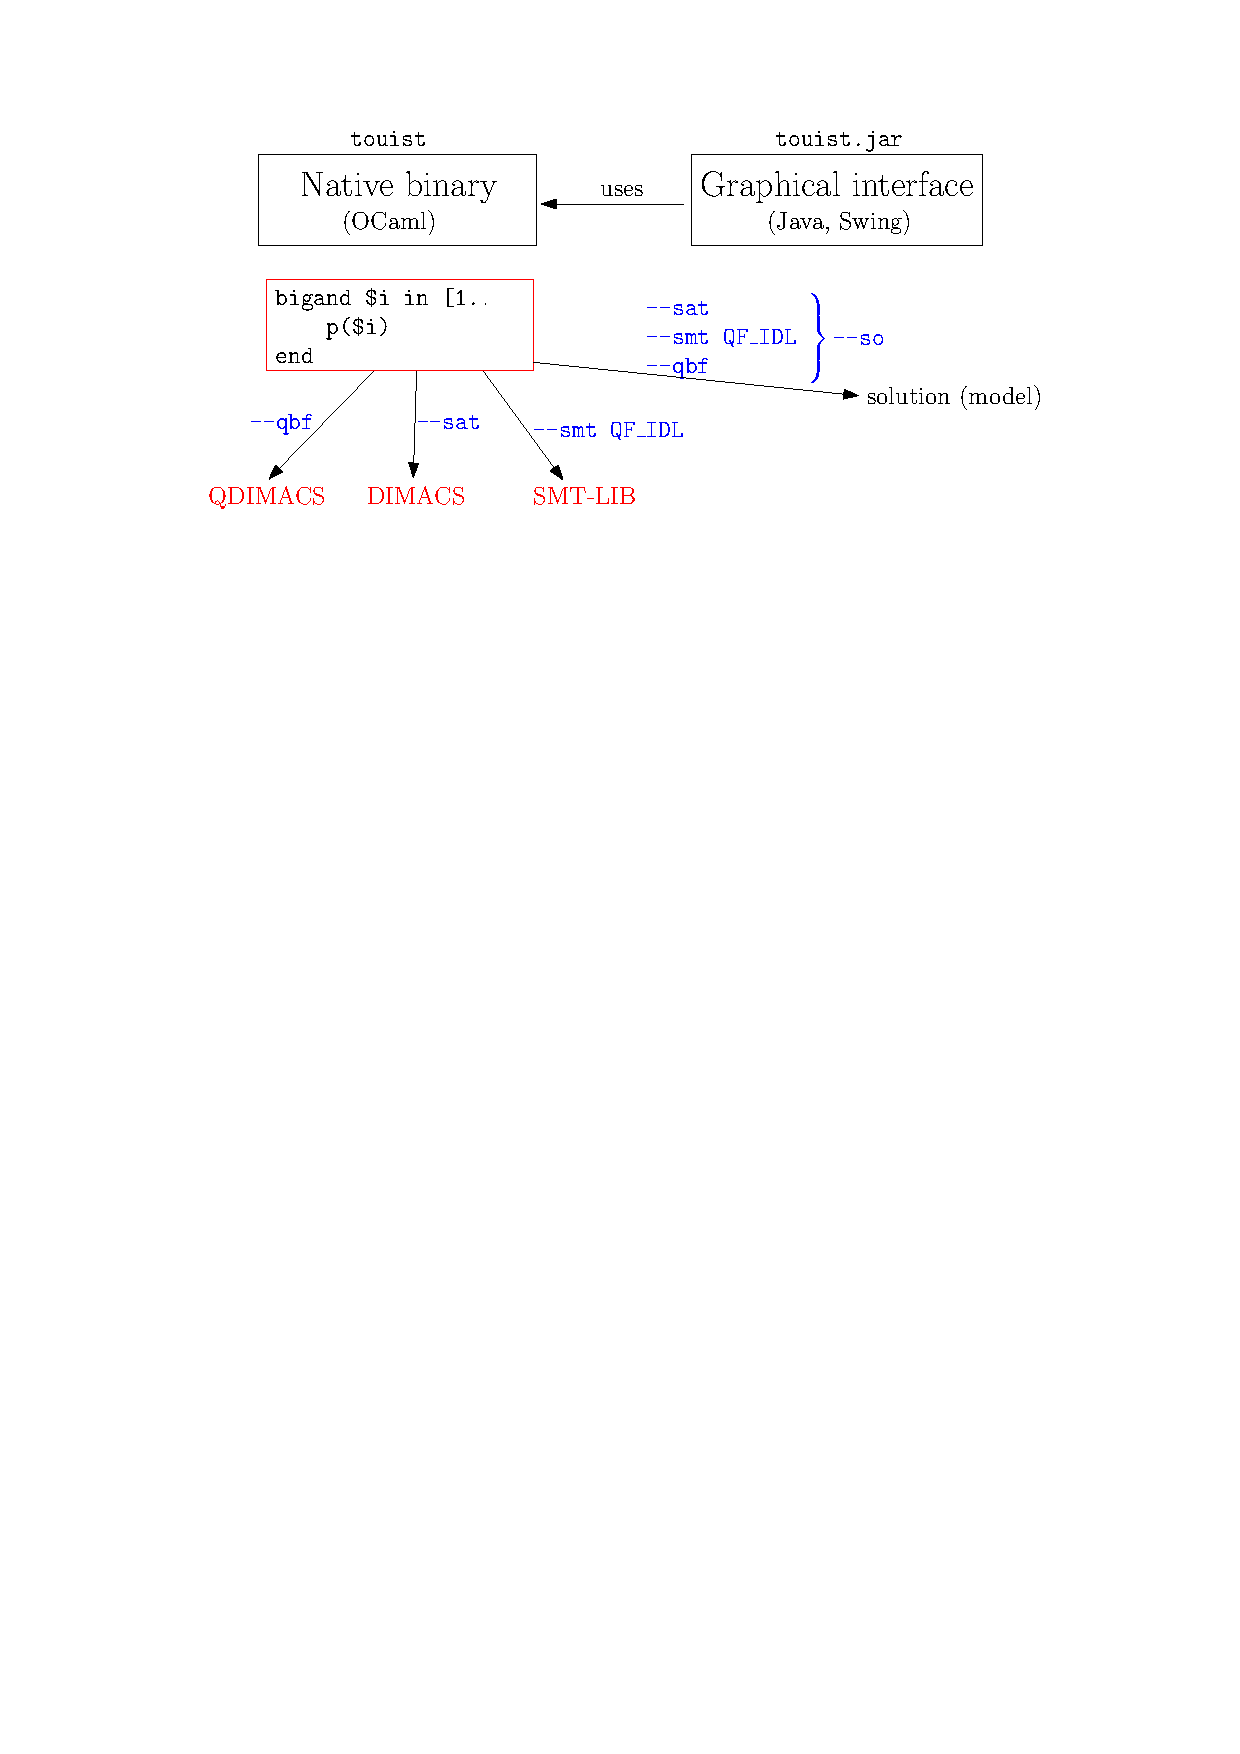
\includegraphics[keepaspectratio=true,width=\dimwidth{1.00}]{figures/architecture}{}}%mdk


\subsection{Usage}\label{cli}%mdk%mdk

\noindent Any \mdcode{touist} command is of the form:%mdk
\begin{mdpre}%mdk
\noindent\preindent{4}touist~{}[-o~OUTPUT]~(INPUT~\textbar{}~-)~{}[options...]%mdk
\end{mdpre}\noindent The flags can be given in any order. You can use the standard input
(\mdcode{stdin}) instead of using an input file by setting the \mdcode{-} argument.
With no \mdcode{-o} flag, \mdcode{touist} will output to the standard output (\mdcode{stdout}).

The man page of \mdcode{touist} is available through \mdcode{man~touist} or \mdcode{touist~--help}.
It contains almost everything you need to know its features and arguments.%mdk

\subsubsection{Exit status}\label{sec-exit-status}%mdk%mdk
\begin{mdtabular}{3}{\dimeval{(\linewidth)/3}}{1ex}%mdk
\begin{tabular}{cll}\midrule
{\bfseries Code}&\multicolumn{1}{c}{{\bfseries Label}}&\multicolumn{1}{c}{{\bfseries Description}}\\

\midrule
0&\mdcode{OK~~~~~~~~~~~~~}&with \textendash{}solve or \textendash{}solver, means SAT\\
8&\mdcode{UNSAT~~~~~~~~~~}&with \textendash{}solve or \textendash{}solver, means UNSAT\\
50&\mdcode{TRANSL\_ERROR~~~~~~}&any error of syntax, type or during the translation\\
100&\mdcode{SOLVER\_ERROR}&any solver error (memory overflow, wrong something\dots{})\\
124&\mdcode{CLI\_ERROR~~}&something wrong with the command-line arguments\\
125&\mdcode{BUG~~~}&the solver did not find any model\\
9&\mdcode{SOLVER\_UNKNOWN~}&\\
\midrule
\end{tabular}\end{mdtabular}

\noindent Note that the \mdcode{UNSAT} is not really an error, but we choose to return a
non-zero exit status anyway.%mdk

\subsubsection{Usage for propositional logic (SAT mode)}\label{usage-sat}%mdk%mdk

\noindent The language accepted for propositional logic is described in
\ref{sec-propositional-logic-formulas}. This mode is enabled by
default, but can be optionally expressed using the \mdcode{--sat} flag.%mdk

\paragraph{Mapping table for DIMACS output}\label{mapping-table}%mdk%mdk

\noindent With no other argument, \mdcode{touist} will simply translate the \touist code to
the~\href{http://www.satcompetition.org/2009/format-benchmarks2009.html}{DIMACS} format and then output the mapping table (that maps
each proposition to an integer \textgreater{} 0) in DIMACS comments before the prelude
line (i.e., \mdcode{p~cnf~x~y}; comments must be before the prelude line in the
\href{http://www.satcompetition.org/2009/format-benchmarks2009.html}{DIMACS specification}). For example, if you run:%mdk
\begin{mdpre}%mdk
\noindent\preindent{4}echo~'rain~=\textgreater{}~wet\_road~rain~not~wet\_road'~\textbar{}~touist~-%mdk
\end{mdpre}\noindent you will get the output:
\begin{mdpre}%mdk
\noindent\preindent{4}c~wet\_road~1~~~~~~~~~~\textless{}-~mapping~between~DIMACS~integers~and~propositions\\
\preindent{4}c~rain~2\\
\preindent{4}p~cnf~2~3~~~~~~~~~~~~~\textless{}-~prelude~of~the~DIMACS~file\\
\preindent{4}1~-2~0\\
\preindent{4}2~0\\
\preindent{4}-1~0%mdk
\end{mdpre}\noindent You can redirect this mapping table using the \mdcode{--table~\textless{}filename\textgreater{}} flag.

\paragraph{SAT solver}\label{usage-sat-solver}%mdk%mdk

\noindent By default, \mdcode{touist} embeds~\href{http://minisat.se}{Minisat}
(see~\cite{Sorensson02minisatv1_13}), a SAT solver written in C++ at the
Chalmers University of Technology, Sweden. It is distributed under the
MIT license. To be able to embed it into OCaml, we use the
binding~\href{https://github.com/c-cube/ocaml-minisat}{ocaml-minisat} which relies on a C version of Minisat
(Minisat-C-1.14.1) for portability concerns.%mdk

\textbf{\mdcode{--solve}} asks \mdcode{touist} to solve the SAT problem. By default, the first
model is displayed; you can ask for more models using the \mdcode{--limit~N}
option. The models are separated by lines beginning with \mdcode{====} and for
one model, each line contains a valuation followed by the corresponding
proposition. For example:%mdk
\begin{mdpre}%mdk
\noindent\preindent{4}echo~a~and~b~\textbar{}~touist~-~--solve%mdk
\end{mdpre}\noindent will return a single model (and in this case, there is only one single model):
\begin{mdpre}%mdk
\noindent\preindent{4}1~a\\
\preindent{4}1~b%mdk
\end{mdpre}\noindent Each line corresponds to a valuation, and each valuation should be read
\mdcode{value~proposition}. In the example, $a$ takes the value 1 (true).
With this format, you can easily filter the results. For example,
the following command will only show the propositions that are \mdcode{{\mdcolor{navy}true}}:
\begin{mdpre}%mdk
\noindent\preindent{4}echo~a~and~b~\textbar{}~touist~-~--solve~\textbar{}~grep~\textasciicircum{}1%mdk
\end{mdpre}\noindent**\mdcode{--solve~--interactive} allows the user to display the models one after
the other. Press enter or any other key to continue and \mdcode{q} or \mdcode{n} to stop.

\textbf{\mdcode{--solve~--limit~N}} allows to display multiple models. With this option,
the models are separated by lines beginning with \mdcode{====} and for one model,
each line contains a valuation followed by the corresponding proposition.
For example, with \mdcode{--limit~0} which displays an unlimited number of models:%mdk
\begin{mdpre}%mdk
\noindent\preindent{4}echo~a~or~b~\textbar{}~touist~-~--solve~--limit~0%mdk
\end{mdpre}\noindent will display
\begin{mdpre}%mdk
\noindent\preindent{4}====~model~0\\
\preindent{4}1~a\\
\preindent{4}0~b\\
\preindent{4}====~model~1\\
\preindent{4}0~a\\
\preindent{4}1~b\\
\preindent{4}====~model~2\\
\preindent{4}1~a\\
\preindent{4}1~b\\
\preindent{4}====~found~3~models,~limit~is~0~(--limit~N~for~more~models)%mdk
\end{mdpre}\noindent Note that the model counter begins at 0.

\textbf{\mdcode{--solve~--count}} tries to return the count of models instead of
returning the models. This option will only work for small problems: the
number of models explodes when the number of propositions is big.%mdk

\subsubsection{Other general options}\label{usage-general-options}%mdk%mdk

\noindent The following general options must be using in conjunction of \mdcode{--smt}
, \mdcode{--qbf} or \mdcode{--sat} (\mdcode{--sat} is used by default and can be omitted).%mdk

\textbf{\mdcode{--latex}} translate the given \touist code to $\mbox{\LaTeX}$. Two
options are available:%mdk

\begin{itemize}[noitemsep,topsep=\mdcompacttopsep]%mdk

\item with \mdcode{--latex} (synonym of \mdcode{--latex=mathjax}, only the math formulas
are translated and no header/footer is added (e.g.,
\mdcode{{\mdcolor{navy}\textbackslash{}begin}\{{\mdcolor{navy}document}\}}). This mode is compatible with any
\emph{light} latex processors (e.g., \mdcode{mathjax} or \mdcode{jlatexmath}).%mdk

\item with \mdcode{--latex=document}, a proper header is inserted so that the output can
directly be given to \mdcode{pdflatex} or any other fully-featured latex
processor. The \mdcode{mathtools} package is necessary for
\mdcode{{\mdcolor{navy}\textbackslash{}begin}\{{\mdcolor{navy}pmatrix*}\}} when matching parenthesis span
across multiple lines.%mdk

\item with \mdcode{--latex=katex}, \mdcode{{\mdcolor{navy}\textbackslash{}substack}\{\}} is replaced by
\mdcode{{\mdcolor{navy}\textbackslash{}begin}\{{\mdcolor{navy}matrix}\}}.%mdk
%mdk
\end{itemize}%mdk

\noindent\textbf{\mdcode{--show=AST}} outputs the AST or translation steps; AST can be
- \mdcode{form} shows the formula generated by the given \touist file. This
   is useful for debugging and testing that the constructs \mdcode{{\mdcolor{navy}bigand}},
   \mdcode{{\mdcolor{navy}bigor}}, \mdcode{{\mdcolor{navy}exact}}\dots{} are correclty evaluated.
- \mdcode{cnf} shows the AST after the CNF transformation (warning: huge).
- \mdcode{duringcnf} shows the recursive translation steps leading to the
   CNF AST.
- \mdcode{prenex} and \mdcode{duringprenex} are similar to the two previous ones
   but for prenex transformation (only with \mdcode{--qbf}).%mdk

\textbf{\mdcode{--show-hidden}} is specific to the SAT mode. When displaying the
DIMACS result, also include the hidden propositions that have been
generated during the CNF expansion by the~\href{https://en.wikipedia.org/wiki/Conjunctive_normal_form}{Tseitin} transformation.%mdk

\noindent\textbf{\mdcode{--linter}} disables all outputs except for errors. It also shortens
then evaluation step by bypassing the expansive \mdcode{{\mdcolor{navy}bigand}}, \mdcode{{\mdcolor{navy}exact}},
\mdcode{{\mdcolor{navy}powerset}}\dots{} constructs.%mdk

\textbf{\mdcode{--error-format}} allows the user to format the errors as you wish.
This argument can be useful for plugging \mdcode{touist} to another program that
needs to read the errors. The placeholders you can use are:%mdk
\begin{mdtabular}{2}{\dimeval{(\linewidth)/2}}{1ex}%mdk
\begin{tabular}{cl}
\midrule
\mdcode{\%f}&file name\\
\mdcode{\%l}&line number (start)\\
\mdcode{\%L}&line number (end)\\
\mdcode{\%c}&column number (start)\\
\mdcode{\%C}&column number (end)\\
\mdcode{\%b}&buffer offset (start)\\
\mdcode{\%B}&buffer offset (end)\\
\mdcode{\%t}&error type (\emph{warning} or \emph{error})\\
\mdcode{\%m}&error message\\
\mdcode{\textbackslash{}n}&new line\\
\midrule
\end{tabular}\end{mdtabular}

\noindent By default, the errors and warnings will display with the formatting
\mdcode{\%f:~line~\%l,~col~\%c-\%C:~\%t:~\%m}. An ending newline (\mdcode{\textbackslash{}n}) is
automatically added.%mdk

\textbf{\mdcode{--wrap-width~N}} lets you choose the width of the messages (errors,
warnings) given by \mdcode{touist}. By default, \mdcode{touist} will wrap all messages with
a 76 characters limit. With N set to 0, you can disable the wrapping.%mdk

\textbf{\mdcode{--verbose}}\mdcode{{}[=N]} or \textbf{\mdcode{-v}}\mdcode{{}[N]} (N defaults to 1) prints more
information on timing and errors. With no N given (i.e., N=1):%mdk

\begin{itemize}[noitemsep,topsep=\mdcompacttopsep]%mdk

\item time spent on translation and solving are displayed (see
table~\ref{timings}).%mdk

\item on syntax error, print more AST context (\mdcode{(loc)} for example).%mdk

\item when an exception is raised, tries to show the stack trace.%mdk

\item on syntax error, print the state number of the LL(1) automaton; each
  state number that may trigger a syntax error should have a
  corresponding message in \mdcode{src/lib/parser.messages}.%mdk
%mdk
\end{itemize}%mdk

\noindent With N \ensuremath{\geq} 2, \mdcode{--solver=CMD} displays the stdin, stdout and stderr of
\mdcode{CMD}.%mdk

\noindent\textbf{Note}.
Availability of timings using \mdcode{-v}:%mdk
\begin{mdtabular}{4}{\dimeval{(\linewidth)/4}}{1ex}%mdk
\begin{tabular}{lccc}\multicolumn{1}{c}{{\bfseries}}&{\bfseries\mdcode{--sat}}&{\bfseries\mdcode{--smt}}&{\bfseries\mdcode{--qbf}}\\

\midrule
\mdcode{translate}&\ding{51}&(instantaneous)&\ding{51}\\
\mdcode{--solve}&\ding{51}&\ding{51}&\ding{51}\\
\mdcode{--solver=}&\ding{51}&(cmd not available)&\ding{51}\\
\end{tabular}\end{mdtabular}
\label{timings}%mdk%mdk

\subsubsection{Usage for Satisfiability Modulo Theory (SMT mode)}\label{usage-smt}%mdk%mdk

\noindent The language accepted by the SMT mode is described in~\ref{sec-smt-formulas}.%mdk

By default, \mdcode{touist} is able to translate problems into the
\href{http://smtlib.cs.uiowa.edu/language.shtml}{\mdcode{SMT-LIB}} format with the \mdcode{--smt=LOGIC} flag. In this mode,
\mdcode{LOGIC} can be any non-whitespace string of characters (which will be
transformed in uppercase automatically). \mdcode{LOGIC} will simply be used
to fill the correct field in the \mdcode{SMT-LIB} file.%mdk

\paragraph{SMT solver}\label{smt-solver}%mdk%mdk

\noindent\touist can embed an optional SMT solver,~\href{http://yices.csl.sri.com}{Yices 2.5.2} (see
\cite{Dutertre:cav2014}). It is developed by SRI (Stanford Research Institute,
California) and is written in C. It is free to use for non-commercial
purposes. Its code is licensed under a restrictive non-commercial EULA
which the user must agree before using (see the~\href{http://yices.csl.sri.com/yices-newnewlicense.html}{license}). To
enable it, you need to install the OCaml binding~\href{https://github.com/polazarus/ocamlyices2}{\mdcode{yices2}} which
embeds the Yices sources:%mdk
\begin{mdpre}%mdk
\noindent\preindent{4}opam~install~yices2%mdk
\end{mdpre}\noindent If \mdcode{touist} was previously installed, it will be re-installed to support
the newly installed \mdcode{yices2}.

When using both \mdcode{--smt=LOGIC} and \mdcode{--solve}, the \mdcode{LOGIC} argument must be
one of~\href{http://yices.csl.sri.com/doc/smt-logics.html}{the logics} Yices 2.5.2 supports. Here is a table
with the logics that are can be used through the \touist language:%mdk
\begin{mdtabular}{2}{\dimeval{(\linewidth)/2}}{1ex}%mdk
\begin{tabular}{ll}\multicolumn{1}{c}{{\bfseries\mdcode{LOGIC}}}&\multicolumn{1}{c}{{\bfseries Meaning}}\\

\midrule
\mdcode{QF\_IDL}&Integer Difference Logic\\
\mdcode{QF\_RDL}&Real Difference Logic\\
\mdcode{QF\_LIA}&Linear Integer Arithmetic\\
\mdcode{QF\_LRA}&Linear Real Arithmetic\\
\end{tabular}\end{mdtabular}

\noindent Note that \emph{QF} means quantifier-free. Also note that you can solve any
SAT problem using any SMT logic solver.%mdk

For example:%mdk
\begin{mdpre}%mdk
\noindent\preindent{4}echo~'x~\textgreater{}~3'~\textbar{}~touist~--smt=QF\_IDL~--solve~-%mdk
\end{mdpre}\noindent which will give you the model
\begin{mdpre}%mdk
\noindent\preindent{4}4~x%mdk
\end{mdpre}\noindent which should be read as $x$ takes the value 4.

\subsubsection{Usage for quantified boolean logic (QBF mode)}\label{usage-qbf}%mdk%mdk

\noindent For now, the \mdcode{QDIMACS} format (which is the equivalent of \mdcode{DIMACS} for
quantified boolean formulas) cannot be printed from a \touist file.
You can still solve problems using both \mdcode{--qbf} and \mdcode{--solve}
(see~\mdref{usage-qbf-solver}{below} section).%mdk

\paragraph{QBF solver}\label{usage-qbf-solver}%mdk%mdk

\noindent\mdcode{touist} can embed an optional QBF solver,~\href{http://fmv.jku.at/quantor/}{Quantor 3.2} (see
\cite{Biere2004}). It is developed at the Johannes Kepler University, Austria.
Its source is under a (non-restrictive) BSD license. To enable the QBF
solver, you must install the OCaml binding~\href{https://github.com/c-cube/ocaml-qbf}{\mdcode{qbf}} which embeds
the Quantor source:%mdk
\begin{mdpre}%mdk
\noindent\preindent{4}opam~install~qbf%mdk
\end{mdpre}\noindent Then, we can solve a small example:
\begin{mdpre}%mdk
\noindent\preindent{4}echo~'forall~x:~x~or~(exists~y:~y)'~\textbar{}~touist~--qbf~--solve~-%mdk
\end{mdpre}\noindent which will give you a partial model:
\begin{mdpre}%mdk
\noindent\preindent{4}?~x\\
\preindent{4}?~y%mdk
\end{mdpre}\noindent where \mdcode{?} means that this value is undefined. To get an actual mode, we
must \emph{force} the valuations (and doing so, we explore the tree of possible
valuations). \mdcode{touist} and its graphical interface are unable to force these
valuations and explore the tree. As a consequence, they are also unable
to visualize the tree (where each leaf would be a model). For now, the only
way to do it is by hand.

\subsection{Using external solvers from \mdcode{touist} (\mdcode{--solver})}\label{sec-using-external-solvers-from-touist---solver}%mdk%mdk

\noindent Most SAT and QBF solvers accept the standardized~\href{http://www.satcompetition.org/2009/format-benchmarks2009.html}{DIMACS} (resp.
QDIMACS) as input language. You can give the DIMACS output of \mdcode{touist}
directly to the solver and use the mapping table (see Section~\ref{mapping-table}).
But you can use \touist to do both the call to the solver as well as the
translation of the resulting DIMACS model back to propositions names, using
the argument \mdcode{--solver}:%mdk
\begin{mdpre}%mdk
\noindent\preindent{4}touist~{}[--sat\textbar{}--qbf]~--solver="\textless{}cmd-and-arguments\textgreater{}"~{}[--verbose]%mdk
\end{mdpre}\noindent For debugging purposes, you can add \mdcode{--verbose} to see the stdin/stdout/stderr.
The exit code of \mdcode{touist} is the same as with \mdcode{--solve}.

The external solvers must use the following Minisat + (Q)DIMACS conventions:
- should accept DIMACS or QDIMACS on standard input;
- should print a model (or a partial model) in DIMACS on standard output; the
  model can span on multiple lines, each line begins with \mdcode{v}, \mdcode{V}
  or nothing (for Minisat compatibility), and each line is optionally ended
  with 0.%mdk
\begin{mdpre}%mdk
\noindent\preindent{2}v~-1~2~-3~4~0\\
\preindent{2}v~5~-6~0%mdk
\end{mdpre}
\begin{itemize}[noitemsep,topsep=\mdcompacttopsep]%mdk

\item should return 10 (as error code) if problem is SAT, 20 if UNSAT.%mdk
%mdk
\end{itemize}%mdk

\noindent Tested SAT solvers (\mdcode{brew} is available on~\href{http://linuxbrew.sh}{linux} and~\href{https://brew.sh}{mac}):%mdk

\begin{itemize}%mdk

\item{}
\href{http://minisat.se}{minisat}%mdk
\begin{mdpre}%mdk
\noindent brew~install~minisat\\
touist~test/sat/sudoku.touist~--solver="minisat~/dev/stdin~/dev/stdout"%mdk
\end{mdpre}%mdk

\item{}
\href{http://fmv.jku.at/picosat}{picosat} (2015, version 965, SAT Race'15)%mdk
\begin{mdpre}%mdk
\noindent brew~install~touist/touist/picosat\\
touist~test/sat/sudoku.touist~--solver="picosat~--partial"%mdk
\end{mdpre}%mdk

\item{}
\href{https://www.labri.fr/perso/lsimon/glucose}{glucose} (2016, version 4.1, syrup is the parallel version)%mdk
\begin{mdpre}%mdk
\noindent brew~install~touist/touist/glucose\\
touist~test/sat/sudoku.touist~--solver="glucose~-model"\\
touist~test/sat/sudoku.touist~--solver="glucose-syrup~-model"%mdk
\end{mdpre}%mdk
%mdk
\end{itemize}%mdk

\noindent Tested QBF solvers:%mdk

\begin{itemize}%mdk

\item{}
\href{https://www.react.uni-saarland.de/tools/caqe/index.html}{caqe} (2017-07-19, CAQE qbfeval 2017, binary release without certification).
Download the version \emph{CAQE qbfeval 2017 (2017-07-19) binary release without certification}
which will give you \mdcode{caqe-mac}:%mdk
\begin{mdpre}%mdk
\noindent touist~test/qbf/allumettes2.touist~--qbf~--solver="./caqe-mac~--partial-assignments"%mdk
\end{mdpre}
They also have a Homebrew tap repository but this version does not contain
the needed \mdcode{--partial-assignments}.%mdk%mdk

\item{}
\href{https://github.com/perebor/qute}{qute} (2017-02-27, fork maelvalais/qute, minisat-based)%mdk
\begin{mdpre}%mdk
\noindent brew~install~touist/touist/qute\\
touist~test/qbf/allumettes2.touist~--qbf~--solver="qute~--partial-certificate"%mdk
\end{mdpre}%mdk

\item{}
\href{http://lonsing.github.io/depqbf/}{depqbf} (2017-08-02, DepQBF 6.03, Minisat-based QCDCL)%mdk
\begin{mdpre}%mdk
\noindent brew~install~depqbf\\
touist~test/qbf/allumettes2.touist~--qbf~--solver="depqbf~--qdo~--no-dynamic-nenofex"%mdk
\end{mdpre}%mdk

\item{}
\href{http://fmv.jku.at/quantor/}{quantor} (2014-10-26, Quantor 3.2). It is not necessary to use this
solver externally as it is included with \mdcode{touist} (see Section~\ref{usage-qbf-solver}).%mdk
\begin{mdpre}%mdk
\noindent brew~install~touist/touist/quantor\\
touist~test/qbf/allumettes2.touist~--qbf~--solver="quantor"%mdk
\end{mdpre}%mdk

\item{}
\href{http://sat.inesc-id.pt/~mikolas/sw/areqs/}{rareqs} (2012, v1.1, CEGAR)%mdk
\begin{mdpre}%mdk
\noindent brew~install~touist/touist/rareqs\\
touist~test/qbf/allumettes2.touist~--qbf~--solver="rareqs"%mdk
\end{mdpre}%mdk
%mdk
\end{itemize}%mdk

\section{Technical details}\label{sec-technical-details}%mdk%mdk

\subsection{One single syntax error per run}\label{sec-one-single-syntax-error-per-run}%mdk%mdk

\noindent You might have noticed that on every run of \mdcode{touist}, only one error is
shown at a time. Many compilers are able to show multiple errors across
the file (e.g., any C compiler). Some other compilers, like OCaml, only
display one error at a time. This feature is often expected by developers
as a time saver: one single run of the compiler to squash as many
mistakes as possible.%mdk

This feature is tightly liked to one particular trait of the grammar of
the language: the semi-colon (\mdcode{;}). When an error comes up, the
semi-colon will act as a checkpoint to which the parser will try to skip
to. Hoping that this error is only contained in this instruction, the
parser will try to continue after the semi-colon.%mdk

The \touist grammar does not have such an instruction marker; because of
that, we are not able to skip to the next instruction.%mdk